\chapter{Implementación sobre Qanus}
\label{chap:qanus} \label{chap:5}
\faltadependiente
En este capitulo veremos la implementación del modelo de question answering multilingüe y diferentes evaluaciones realizadas utilizando como guía dos tareas monolingües de la competencia QA@Clef '07, una para español y otra para portugués. El sistema está basado en un framework académico de código abierto llamado Qanus. Este framework está empaquetado con una sistema de QA simple, QA-sys, que resuelve ejercicios de la competencia Trec '07 con soporte para inglés. Nosotros adaptamos este sistema para utilizar como librería de procesamiento de lenguajes a Freeling, generando un sistema baseline multilingüe. A este sistema le agregamos features reseñados en \allref{sec:literatura} y realizamos diferente mediciones sobre las instancias en español y portugués sobre los ya mencionados ejercicios de Clef '07.

La estructura de este capitulo es la siguiente: en \allref{sec:ejercicio-de-clef} se describe con detalle el panorama general de tareas de question answering en la competencia Clef '07, haciendo énfasis en las tareas seleccionadas, en los corpus y las preguntas disponibles y en las decisiones tomadas a la hora de elegir estas tareas; en \allref{sec:sistema} se comenta la adaptación del sistema baseline y las modificaciones realizadas a los algoritmos, {\color{red}mientras que los resultados pueden observarse como apartados en las mismas secciones o como una sección aparte al final}.

\section{Ejercicio de Clef}
\label{sec:ejercicio-de-clef}
Tras investigar distintas competencias y métodos de evaluación, optamos por utilizar como guía de trabajo dos ejercicios de la tarea principal de question answering de la competencia Clef de 2007. Principalmente por contar con un subconjunto de ejercicios bastante adecuados para nuestra tesis y disponer de un corpus de datos libre y disponible en el acto para evaluar una parte importante de las funcionalidades implementadas en nuestro proyecto.

Como mencionamos en \allref{subsec:competencias}, Clef (de \textit{Cross-Language Evaluation Forum}) es una organización que busca fomentar la investigación en sistemas de information retrieval cross-language. En particular, una vez por año Clef lanza una competencia de Question Answering multilingüe, con diferentes corpus y diferentes tipos de ejercicios. Estas competencia permiten obtener un patrón estándar de comparación entre distintos desarrollos y una idea general del estado de arte alcanzado en los diferentes idiomas por la diferentes actores académicos y comerciales. Por lo demás, Clef es el principal organizador de conferencias de question answering multilingüe para idiomas europeos y la tarea principal de '07 presentaba una complejidad adecuada para el scope de esta tesis.

La competencia de 2007 es la quinta campaña de QA multilingüe de Clef, siendo la primera en 2003.

La tarea estándar principal de question answering incorpora algunas particularidades que la diferencian de anteriores campañas: los temas o tópicos, la co-referencia y el uso de wikipedia como corpus de datos parcial. Además de la tarea principal se presentaron tres tareas más: Answer Validation Exercise (AVE) y QUAST, question answering in speech transcription y Question Answering Real Time, con métricas de performance temporales. Como nota general, es importante notar que las tareas fueron de una complejidad elevada y en comparación con los resultados del año anterior, la mejor precisión general bajó del 49\% al 41.75\% para tareas multi-lingües, mientras que, más significativamente, bajó de 68\% a 54\% en tareas monolingües.


\subsection{Tareas}
\label{subsec:tareas}
Utilizamos como guía dos ejercicios de la tarea principal de question answering de '07  por varias razones (Ver \cite{GuidelineClef07} y \cite{OverviewClef07} para un detalle exhaustivo de la conferencia en cuestión). Para esta tarea estaban disponibles en acto corpus, inputs de prueba y resultados esperados para una experimentación multilingüe que abarque tanto inglés como español y portugués. Además, estos ejercicios incorporaban, por única vez, diferentes wikipedias como parte del corpus de datos, lo cual resulta de por si atractivo.

La tarea principal de QA de Clef '07 ofrece dos grandes grupos de ejercicios:
\begin{itemize}
\item Mono-lingual: donde el idioma de la pregunta y el idioma de la fuente de información son el mismo
\item Cross-lingual: donde el idioma de la pregunta y el idioma de la fuente de información difieren
\end{itemize}

En ambos grupos, los sistemas reciben un set de 200 preguntas - que pueden ser de hechos o eventos (factoid), definiciones de personas, cosas u organizaciones (definition), listas de personas, objetos o datos (list) - y se exige devolver una respuesta exacta, donde exacta significa sin más información de la mínima necesaria. Siguiendo el ejemplo de Trec, los ejercicios de este año contienen topics, i.e. clusters de preguntas relacionadas con un mismo tema y con posibilidad de co-referencia entre las preguntas del grupo. Ni el tipo de la pregunta ni el tópico es dado a los participantes.

La respuesta tiene que estar soportada por el id del documento del cual se extrajo y por la porción de texto que proveyó contexto suficiente para soportar la corrección de la respuesta. Los “textos de soporte” pueden venir de diferentes partes de documentos relevantes y deben sumar un máximo de 700 bytes. No hubo restricciones sobre la longitud del string de respuesta, pero fragmentos de información innecesaria fueron penalizados marcando la respuesta como ineXacta.

Otra particularidad de los ejercicios es que hay preguntas sin respuesta en el corpus que esperan como respuesta 'Nil'.


Se consideraron 10 idiomas para preguntas: búlgaro, holandés, inglés, francés, alemán, indonesio, italiano, portugués, romano y español. Todos estos idiomas se usaron como idiomas del corpus, a excepción del indonesio para el que no se disponía de una colección de noticias.

Se propusieron, en total, 37 tareas concretas: 8 monolingües y 29 bilingües. Dada la complejidad de la construcción del ejercicio mismo, la organización solo implementó concretamente las tareas tomadas por algún equipo competidor.


\begin{figure}
  \centering
    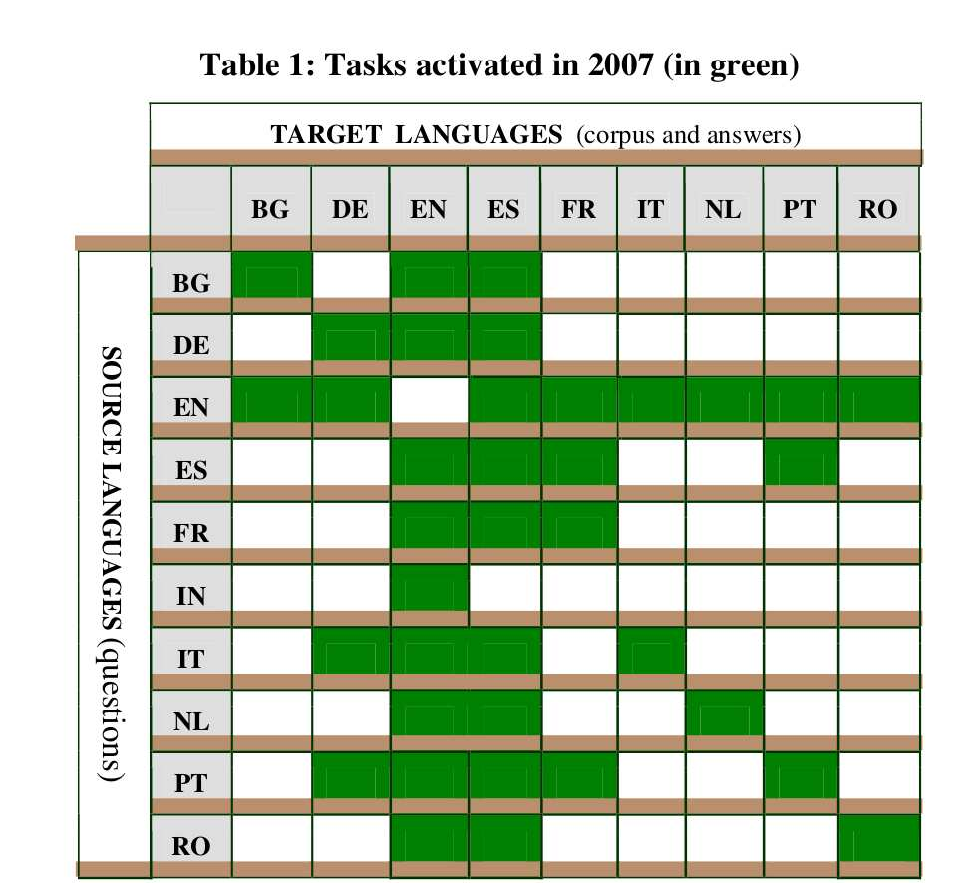
\includegraphics[scale=0.5]{graficos/clef07}
  \caption{Tareas activadas en la competencia Clef '07}
  \label{fig:tareas}
\end{figure}

El corpus de datos propuesto consiste en dos corpora distintos: una serie de de recopilados específicamente por los organizadores de la competencia y utilizado con frecuencia en competencias anteriores y, por otro lado, snapshots de las wikipedias en diferentes idiomas con límite en Diciembre de 2006.

Para nuestro proyecto utilizamos las preguntas y los datos de evaluación de los ejercicios monolingües es-es (español-español) y pt-pt (portugués-portugués) implementando como corpus de datos solo las wikipedias.

Los datos de los ejercicios constan de dos archivos: un archivo con 200 preguntas agrupadas por temas y otro archivo con diferentes traducciones de la pregunta, una respuesta goldstandard con soporte textual y el id del documento de soporte para el idioma target (del corpus).

Por otro lado, en la guía de ingreso a la competencia\cite{GuidelineClef07} se proveen links para descargar los snapshots de wikipedia sugeridos. Se ofrece una versión de wikipedia en inglés preprocesada de Noviembre de 2006 \footnote{\url{http://ilps.science.uva.nl/WikiXML/}}, dos opciones para descargar wikipedia en español: una imagen estática en html de Noviembre de 2006 \footnote{\url{http://static.wikipedia.org/downloads/November_2006/es/}} y un dump xml de Diciembre de 2006 \footnote{\url{http://download.wikimedia.org/images/archive/eswiki/20061202/pages-articles.xml.bz2}} y también X opciones de portugués.

La guía aclara que, bajo responsabilidad de los participantes, se puede usar
cualquier otra versión de Wikipedia, siempre y cuando sea anterior a noviembre / diciembre de 2006.
Además, se pide que las respuestas sean tomadas de ``entradas reales" o artículos de wikipedia y
no de otros documentos (imágenes, discusión, categoría, template, histórico de revisiones, datos de usuario y páginas con meta información).

Los links a páginas de wikipedia en español y en portugués no estaban más disponibles (ambos respondieron 404), mientras que el formato
preprocesado pedido para el inglés resultaba realmente complejo de instalar y parecía una linea muerta. Por estos motivos,
seguimos la sugerencia sobre el uso responsable de otras wikipedias y utilizamos las siguientes snapshots de Wikidumps\footnote{Ver \url{http://dumps.wikimedia.org/} y \url{http://en.wikipedia.org/wiki/Wikipedia:Database_download\#Other_languages}}.

\begin{center}
\begin{tabular}{ | l | l | l | l |}
    \hline
    Idioma & Fecha & Tamaño & \# Entradas \\ \hline
    Español & 5 de Julio de 2006 & 558M  & 233750  \\ \hline
    Portugués & 1 de Febrero de 2007 & 776M  & 498039  \\ \hline
    Inglés Simple & 4 de Julio de 2006 & 26M   & 18273   \\ \hline
    Inglés & 4 de Noviembre de 2006 & 7,6G  &   \\ \hline
    Español & 26 de Enero de 2007 & 902M  &   \\ \hline
    Español & 14 de Junio de 2013 & 7,3G  &   \\ \hline
    Inglés Simple & 24 de Julio de 2013 & 406M  &   \\ \hline
\end{tabular}
\end{center}

Utilizando la información disponible en los archivos de respuestas esperadas, discriminamos las preguntas con respuestas con soporte de wikipedia, las soportadas por el corpora de noticias de la organización y las que no tienen respuesta (NIL):

\begin{center}
\begin{tabular}{| l | l | l | l | l |}
\hline
Idioma & Wiki & News & NIL & Total \\ \hline
es & 155 & 37 & 8 & 200 \\ \hline
pt & 130 & 59 & 11 & 200 \\ \hline
\end{tabular}
\end{center}


\subsection{Análisis de las preguntas}

Las 200 preguntas del test set están agrupadas por tema, y cada tema tiene de una a cuatro preguntas. Los temas pueden ser entidades nombradas, evento o también categorías como objetos, fenómenos naturales, etc (por ejemplo: Bush, Juegos Olímpicos, notebooks, huracanes, etc).
Los temas no están dados en el set de test, pero pueden ser inferidos del primer par pregunta respuesta. La relación del tema con el grupo de preguntas respetaba las siguiente condiciones:

\begin{itemize}
\item El tema es nombrado en la primer pregunta o bien en la primera respuesta.
\item Las siguientes preguntas pueden contener co-referencias al tema expresado en el primer par pregunta/respuesta
\end{itemize}


Para ilustrar el punto consideremos el primer grupo de preguntas para el ejercicio de español es:
\begin{itemize}
\item ¿En qué colegio estudia Harry Potter?
\item ¿Cuál es el lema del colegio?
\item ¿En qué casas está dividido?
\item ¿Quién es el director del colegio?
\end{itemize}


Como ya mencionamos, algunas preguntas podían no tener respuesta en la colección de documentos, y en ese caso la respuesta exacta era “NIL” y la justificación y el docid vacíos. La organización definió como criterio de inexistencia de la respuesta que ni los asesores humanos ni los demás sistemas participantes pudieran encontrar alguna.

En lo que respecta a los tipos de pregunta, el ejercicio considerara tres categorías: Factoid, Definition y Closed List.

\begin{center}
\begin{table}
\begin{tabular}{| l |  p {12cm} |}
\hline
Tipo & Descripción  \\ \hline
FACTOID & preguntas fácticas, preguntando el nombre de una persona, un lugar, la medida de algo, el día en que algo ocurrió, etc. \\ \hline
DEFINITION & preguntas como Qué/ Quién es X? \\ \hline
CLOSED LIST & questions that require one answer containing a determined number of items, e.g \\ \hline
\end{tabular}
\caption{Definición de los tipos de pregunta}
\label{table:question-type-definition}
\end{table}
\end{center}

Todos los tipos de pregunta podían contener restricciones temporales, i. e: una especificación temporal proveyendo importante información para devolver una respuesta correcta. Por ejemplo: \newline
Q: Who was the Chancellor of Germany from 1974 to 1982? \newline
A: Helmut Schmidt.\newline
Q: Which book was published by George Orwell in 1945?\newline
A: Animal Farm.\newline
Q: Which organization did Shimon Perez chair after Isaac Rabin’s death?\newline
A: Labour Party Central Committee.\newline


%Los calculos propios coinciden con el análisis presentado en \cite{OverviewClef07} en la siguiente discriminación del total de preguntas en función de las categorías recién señaladas:
\begin{center}
\begin{table}[H]
\centering
\begin{tabular}{| l | l | l | l | l | l |}
\hline
Subset & Idioma & Factoid & Definition & List & Total \\ \hline
\multirow{2}{*}{Todo} & es & 158 & 32 & 10 & 200 \\ \cline{2-6}
 & pt & 159 & 31 & 10 & 200 \\ \hline
 \multirow{2}{*}{Wiki} & es & 122 & 24 & 9 & 155 \\ \cline{2-6}
 & pt & 104 & 18 & 8 & 130 \\ \hline
\end{tabular}
\caption{Totales por tipo de pregunta}
\label{table:totals-type-question}
\end{table}
\end{center}

Los tipos de preguntas disponen a su vez de subtipos. Las preguntas factoid disponen de 8 subtipos, las de definiciones y listas tienen 4.
Se consideraron los siguiente 8 tipos de Factoids:

\begin{center}
\begin{table}[H]
\centering
\begin{tabular}{| l | p{12cm}|}
\hline
Tipo & Ejemplo \\ \hline
PERSON &  Q: Who was called the \dq{Iron-Chancellor}? \newline A: Otto von Bismarck. \\ \hline
LOCATION & Q: Which town was Wolfgang Amadeus Mozart born in? \newline A: Salzburg. \\ \hline
ORGANIZATION & Q: What party does Tony Blair belong to? \newline A: Labour Party.\\ \hline
MEASURE &Q: How high is Kanchenjunga?\newline A: 8598m. \\ \hline
COUNT & Q: How many people died during the Terror of Pol Pot? \newline A: 1 million.\\ \hline
OBJECT & Q What does magma consist of?\newline A: Molten rock.\\ \hline
TIME & Q: What year was Martin Luther King murdered?\newline A: 1968.\\ \hline
OTHER & i.e. todo lo que no encaja en las categorías anteriores.\newline Q: Which treaty was signed in 1979? \newline
A: Israel-Egyptian peace treaty.\\ \hline
\end{tabular}
\caption{Tipos de respuesta esperada para preguntas Factoid}
\label{table:type-factoid}
\end{table}
\end{center}

Las preguntas de tipo LIST consisten son enumeraciones de 4 tipos posibles: PERSON, LOCATION, ORGANIZATION y OTHER.
Por ejemplo:\newline
Q: Name all the airports in London, England. \newline
A: Gatwick, Stansted, Heathrow, Luton and City.

Como solo una fuente estaba estaba permitida, los items debían aparecer en secuencia, uno después del otro, en uno documento de la colección .
Con respecto a las preguntas de tipo definition, también cuatro tipos, con otra semántica.


\begin{center}
\begin{table}[H]
\centering
\begin{tabular}{| l | p{12cm}|}
\hline
Tipo & Descripción y ejemplo \\ \hline
PERSON & i.e. preguntas sobre el rol, el trabajo o información importante de alguien \newline
 Q: Who is Robert Altmann? \newline
 A: Film maker. \\ \hline
ORGANIZATION & i.e. preguntas sobre la misión, el nombre completo o información relevante sobre una organización \newline
 Q: What is the Knesset? \newline
 A: Parliament of Israel. \\ \hline
OBJECT & i.e. preguntas por la descripción o función de objetos \newline
Q: What is Atlantis? \newline
A: Space Shuttle. \\ \hline
OTHER & i.e. preguntas por descripciones de fenómenos naturales, tecnologías, procedimientos legales, etc. \newline
Q: What is Eurovision? \newline
A: Song contest. \\ \hline
\end{tabular}
\caption{Tipos de respuesta esperada para preguntas Definition}
\label{table:definition-questions}
\end{table}
\end{center}

\begin{center}
\begin{table}[H]
\centering
\begin{tabular}{| l | l | l | l | l | l |l |l|l|}
\hline
Tipo & pt & es & pt-factoid & es-factoid & pt-def & es-def & pt-list & es-list \\ \hline
COUNT & 21 & 22 & 21 & 22 & 0 & 0 & 0  & 0\\ \hline
OBJECT & 11 & 27 & 6  & 18 & 5 & 9 & 0  & 0\\ \hline
MEASURE & 15 & 20 & 15 & 20 & 0 & 0 & 0  & 0\\ \hline
PERSON & 33  & 35 & 21 & 24 & 9 & 8 & 3 & 3\\ \hline
TIME & 19 & 16 & 18 & 16 & 0 & 0 & 1 & 0\\ \hline
LOCATION & 33 & 18  & 30 & 18 & 0 & 0 & 3 & 0 \\ \hline
ORGANIZATION & 31 & 32 & 24 & 22 & 6 & 8 & 1 & 2\\ \hline
OTHER & 37 & 30 & 24 & 18 & 11 & 7 & 2 & 5 \\ \hline
Total & 200 & 200 & 159 & 158 & 31 & 32  & 10 & 10\\ \hline
\end{tabular}
\caption{Tipos de respuesta esperada en función de tipo de pregunta}
\label{table:tipo-general}
\end{table}
\end{center}


\section{Sistema}
\label{sec:sistema}

Nuestra implementación está basada en Qanus como framework o arquitectura de diseño de QA y en Freeling como proveedor de servicios de procesamiento de lenguaje multilingüe. Qanus (Question-Answering @ National University of Singapore) es un framework de question answering basado en information retrieval y también un sistema de QA funcional simple construido sobre este framework. El proyecto se actualizó por última vez en noviembre de 2012 y contiene herramientas actuales de nlp para inglés (el POS-tagger, el NER-tagger y el Question Classifier de Stanford) y también de information retrieval (índice de búsquedas lucene) bajo licencia de código abierto. El paquete cuenta con un framework (qanus), que cumple un rol equivalente a la arquitectura DeepQA en la organización del proyecto de IBM, y un sistema montado sobre este framework -QA-sys-, equivalente a Watson (Ver Figura ~\ref{fig:Quanus}).


\begin{figure}
  \centering
    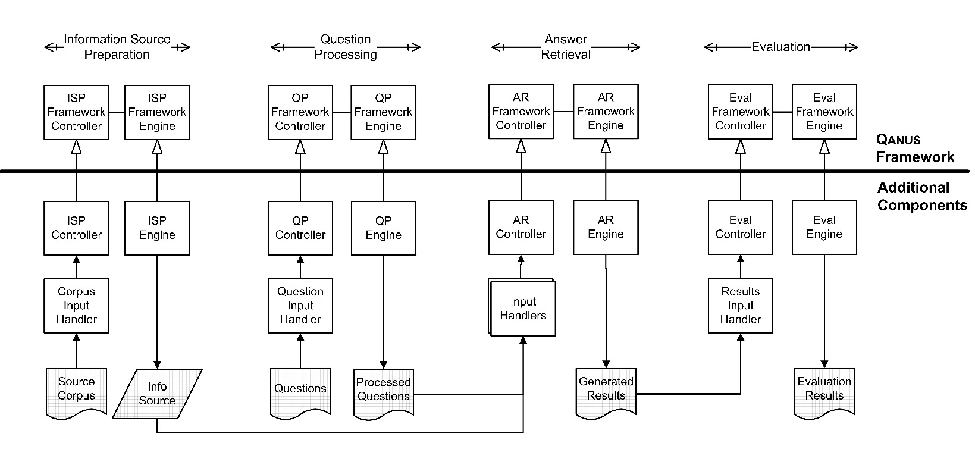
\includegraphics{graficos/Quanus}
  \caption{El framework Quanus y la implementación QA-sys}
  \label{fig:Quanus}
\end{figure}


La arquitectura de Qanus mantiene la estructura de pipeline típica similar a las reseñadas en la sección \allref{chap:estado-de-arte}.
Consta de los siguientes pasos: \newline

\textbf{Preparación de la fuente de información: } El primer step del pipeline es preprocesar las fuentes de información para un acceso optimizado en pasos posteriores del proceso. La implementación QA-sys incorpora una base de conocimiento en formato XML de aquaint a un índice de
búsquedas Lucene. En este paso se incorpora todo el conocimiento offline; bases de conocimiento dinámicas como la web se modelan en el pasos posteriores. \newline

\textbf{Análisis de la pregunta: } Este paso, igualmente genérico, permite la incorporación de
distintos componentes para anotar los tokens de la pregunta con datos
útiles para ser consumidos por el paso 3. Otro procesamiento a
realizar en este paso podría ser la generación de queries
entendibles por los distintos motores de almacenamientos de
información del paso 1. En particular, la implementación trae un
pos-tagger, un ner-tagger y un question classifier, todos de Stanford.
Hablaremos más de estos componentes más adelante. \newline

\textbf{Generación de respuestas: } En este paso se utiliza la información generada en la preparación
de la base de información y en el procesamiento de la pregunta para
generar una respuesta. También puede incorporarse accesos a la web y
validaciones de las respuestas candidatas. La implementación concreta
evalúa cada pasaje de los primeros n documentos retornados por Lucene
para la pregunta original con una serie de componentes ad-hoc de
distancia para adjudicar diferentes grados de confiabilidad a los
distintos pasajes. \newline


Además, se provee de un cuarto paso opcional (el sistema de QA está
completo con los tres pasos anteriores), para la fase de desarrollo y
de evaluación de la performance del sistema:\newline


\textbf{Evaluación: }Este paso está pensado para evaluar las respuestas generadas y
presentarlas de un modo conciso en la fase de desarrollo.
Básicamente, cruza las respuestas obtenidas contra unas respuestas
esperadas escritas a mano y presenta el total de respuestas dadas
correctamente.\newline

En esta sección de la tesis adoptamos el framework Qanus y adaptamos el sistema QA-sys para 1) incorporar Freeling como librería de herramientas de procesamiento del lenguaje permitiendo un funcionamiento multilenguaje, 2) trabajar sobre el corpus de datos y preguntas de los ejercicios de CLEF '07 de español y portugués descriptos en \allref{sec:ejercicio-de-clef} y, finalmente, 3) incorporamos y evaluamos diferentes mejoras tomadas de la reseña a la literatura científica del apartado anterior \allref{sec:literatura}.

\subsection{Implementación baseline}
\label{subsec:baseline}
El código está escrito en java y mantiene una interfaz común a
todos los pasos: un controller cuyas responsabilidades son cargar los
componentes y un engine que utiliza los componentes para leer el input,
procesarlo y grabar el resultado. La adaptabilidad del framework está
dada en la posibilidad de incorporar componentes respetando la interfaz
especificada para los mismos o bien, en modificar esta misma interfaz.

La implementación QA-sys está desarrollada para correr sobre
el tipo de datos de las evaluaciones Trec 2007.
Brevemente, la implementación realiza las siguientes tareas:
En el primer paso, incorpora los XML en el formato XML Aquaint propuesto por la competencia a un índice Lucene, en
el segundo paso anota la pregunta con POS tags, NERs y
clasifica el tipo de respuesta con un clasificador entrenado y luego,
en el tercer paso se busca la pregunta sobre el índice lucene y se
retorna una lista con n documentos rankeados. Estos documentos se
subdividen en pasajes. Luego se aplican diferente algoritmos ad-hoc
dependiendo del tipo de respuesta esperada. \ Por ejemplo, si la
respuesta es un nombre de persona, se ejecuta NER sobre los diferentes
pasajes buscando nombres candidatos, si el tipo esperado es una fecha,
se utilizan expresiones regulares escritas a mano, etc. Finalmente, los
pasajes candidatos se evalúan utilizando heurísticas de proximidad
de los candidatos a la pregunta inicial. Para esto se utilizan
diferentes Scorers que rankean los pasajes según diferentes
características (features) y luego se selecciona alguna priorizando
algunas características sobre otras, dependiendo también del tipo
de respuesta esperada. Por último, el evaluador de resultados mide la
exactitud (\textit{accuracy}): total de respuestas correctas sobre
total de preguntas.

QA-sys funciona sólo sobre preguntas del tipo
factoid y, a modo de comparación, el mejor sistema según la Trec
2007, el LymbaPA07 obtuvo un grado de exactitud del 0.706 y el décimo
(Quanta) obtuvo 0.206, mientras que QA-sys logra el 0.119 disponiendo de una implementación sumamente simple.

En las siguientes secciones de la tesis describiremos la implementación de nuestro sistema de question answering tomando como base los tres pasos principales del pipeline de QA-sys.

\subsubsection{Base de conocimiento}

El módulo de procesamiento de la base de información de la implementación QA-sys está desarrollada para correr sobre el tipo de datos de las evaluaciones Trec 2007, un formato XML conocido como ``Aquaint". Por otro lado, el mismo framework esta atado al procesador de XMLs SAX, una entre varias implementaciones disponibles en el entorno de java. En nuestra adaptación, incorporamos la librería gwtwiki\footnote{Java Wikipedia API (Bliki engine): \url{http://code.google.com/p/gwtwiki/}} para procesar los xml dumps de wikipedia. Como esta librería no utiliza SAX, nos vimos obligados a modificar el framework.

En este proceso descartamos artículos mal formados y entradas representado imágenes o discusiones, tal como se sugiere en la guía.
Los artículos se indexan en índices Lucene como documentos con los siguiente campos: \emph{id, title, body y all}.
La tabla \ref{table:creacion-indices} muestra algunos datos del proceso de generación de índices, mientras que la figura \ref{fig:LuceneIndexWriterWiki} ilustra el proceso.

Las categorías filtradas contiene artículos con alguno de los siguientes prefijos en el título: WP, wp, Biografías, Wikipedia, Wikiproyecto, Imagen, Plantilla, MediaWiki, Template, Category, Help, Image, Ayuda, Portal, Ajuda, Categoria, Categoría, Imagem, Predefinição.


\begin{table}
\centering
\begin{center}
\begin{tabular}{| l | l | l | l | l | l| l|l|}
\hline
Wikipedia & \# Entradas & Nulas & Redirects & Filtradas & Validas & Tamaño & Tiempo \\ \hline
simple-06 & 18273 & 22 &  3452 & 5241 & 9558 & 26M & 14 secs \\ \hline
es-06 & 233750 & 52 & 62805 & 34947 & 135946 & 558M & 242 secs\\ \hline
pt-07 & 498039 & 80 & 210983 & 43390 & 243586 & 776M & 294 secs\\ \hline
simple-13 & 180067 & 8 & 35600 & 41902 & 102557 & 406M & 133 secs\\ \hline
\end{tabular}
\caption{Datos de procesamiento sobre las diferentes versiones de wikipedia analizadas. Los tiempos de procesamiento están tomados en una Intel Core i3-2100 CPU @ 3.10GHz de dos cores con 8 GiB de RAM.}
\label{table:creacion-indices}
\end{center}
\end{table}


\begin{figure}[H]
  \centering
    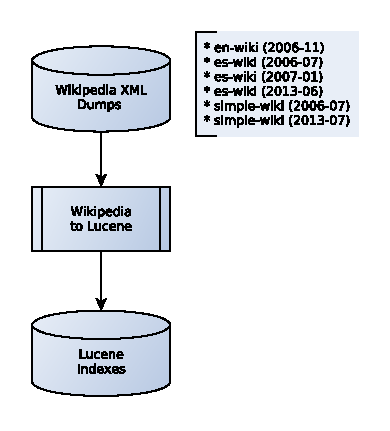
\includegraphics{graficos/LuceneIndexWriterWiki}
  \caption{Lucene Index Writer para dumps de Wikipedia}
  \label{fig:LuceneIndexWriterWiki}
\end{figure}


\subsubsection{Anotado de la pregunta}

El módulo original de QA-sys de procesamiento de la pregunta espera preguntas en el formato Aquaint definido por Trec, al igual que el tipo de datos esperado sobre el corpus en el paso anterior. En el procesamiento lleva a cabo las tareas descriptas de modo general en \allref{subsec:impl-pos}, \allref{subsec:impl-ner} y \allref{subsec:qtype},  utiliza como librerías de procesamiento de lenguaje el POS-Tagger, el NER-Tagger y el Question Classifier de la Universidad de Stanford, disponibles solo para inglés, descriptas en \allref{sec:stanford-both} y \allref{sec:stanford-qc} respectivamente.

En nuestra adaptación incorporamos los módulos de POS y NERC multilingües de freeling. Con respecto a la clasificación de preguntas, ya mencionamos que no existen clasificadores para español y tampoco para el portugués. Frente a esta situación podríamos haber implementado clasificadores heurísticos basados en reglas escritas a mano como en el caso del sistema estructurado (\allref{sec:qp-mitic}). Aprovechando la disponibilidad de una traducción confiable al inglés de las preguntas en archivos de datos (debido a la activación de los ejercicios cross-lingual en-es y en-pt), decidimos utilizar el clasificador de Stanford sobre la traducción inglesa de la pregunta.
Las tablas \ref{table:qc-es} y \ref{table:qc-pt} presentan la distribución de las 200 preguntas para español y para portugués según las seis clases principales del esquema de Li \& Roth.

\begin{table}
\centering
\begin{center}
\begin{tabular}{| l | l | }
\hline
Clase & \# Preguntas  \\ \hline
HUM &  62\\ \hline
NUM &  53\\ \hline
ENTY &  34\\ \hline
DESC &  25\\ \hline
LOC &  24\\ \hline
ABBR &  2\\ \hline
\end{tabular}
\caption{Distribución por clases de las preguntas para el ejercicio monolingüe español}
\label{table:qc-es}
\end{center}
\end{table}



\begin{table}
\centering
\begin{center}
\begin{tabular}{| l | l | }
\hline
Clase & \# Preguntas  \\ \hline
HUM &  53\\ \hline
NUM &  52\\ \hline
ENTY &  28\\ \hline
DESC &  30\\ \hline
LOC &  36\\ \hline
ABBR &  1\\ \hline
\end{tabular}
\caption{Distribución por clases de las preguntas para el ejercicio monolingüe portugués}
\label{table:qc-pt}
\end{center}
\end{table}

Al finalizar este paso, las preguntas tienen asociadas su tipo, las distintas entidades nombradas, el análisis gramatical y las qwords. Dejamos la generación de queries para el paso posterior ya que así es como estaba implementado en el sistema original.

\subsubsection{Generación de Respuestas}

Como baseline de desarrollo y pruebas, adaptamos los algoritmos de Qanus. En esta subsección vamos a describir esta implementación con detalle, mencionando los cambios más importantes que realizamos para adaptarla a la tarea elegida. En las siguientes comentaremos diferentes modificaciones y algoritmia agregada. El proceso de qanus para la generación de respuestas puede estructurarse así:
\begin{enumerate}
  \item Filtrado de preguntas
  \item Generación de Queries
  \item Information Retrieval
  \item Extracción y rankeo de oraciones
  \item POS tagging de las mejores oraciones
  \item Heurísticas de AR basadas en el QC
\end{enumerate}

En el primer paso, se descartan todas las preguntas cuyo tipo no sea \textit{factoid}. Esto, en principio, dejaría afuera a 32 preguntas de tipo \textit{definition} y 10 de tipo \textit{list} para el ejercicio en español (24 y 9, respectivamente, considerando solamente las que como goldstandard answer tienen datos de wikipedia) y 31 de tipo \textit{definition} y 10 de tipo \textit{list} para el portugués (18 y 8, respectivamente, considerando las de wikipedia).

En en segundo paso, la generación de queries, el sistema baseline utiliza 2 algoritmos diferentes según el qtype inferido por el clasificador de preguntas. El primer caso es especifico para la clase fina \sq{HUM:ind} y consta de tres tipos de expresiones regulares escritas a mano y en inglés que matchean contra preguntas de la forma: \dq{Who (is|was) (the)+ NN ... NN?} (NN significa, acá, sustantivo). Por ejemplo: \dq{Who is the CEO of Microsoft?} y \dq{Who VERBO ...?}. En estos casos se extraen los sustantivos y los verbos de la pregunta para generar la query. Eliminamos estos casos ya que adaptarlos a los diferentes idiomas no escalaba para un sistema multilingüe. Por su parte, si el tipo de la pregunta no es \sq{HUM:ind}, el algoritmo general de generación de queries espera, además de la pregunta propiamente dicha, un campo asociado a la pregunta, \sq{target}, aparentemente definido en la competencia TREC para la que está escrito. El campo \sq{target} es utilizado por mucha de la algoritmia que vendrá. Dejaremos en suspenso con qué poblamos ese dato hasta más adelante. Un uso posible es asociarlo el \sq{tópico} del grupo de preguntas de los ejercicios de la competencia. Más adelante veremos qué contenido le cargamos.


El método default FormQuery genera una query que contiene, sin repetir, todas las palabras no-stopwords del campo target y todos los sustantivos, verbos y adjetivos de la pregunta completa según el pos tagger de stanford. Nosotros adaptamos este método para funcionar con las etiquetas de Freeling y utilizamos este mecanismo de generación de queries como baseline.

En el tercer paso, a partir de la query generada, se hace un pedido al índice lucene. En el cuarto paso, los documentos son divididos en oraciones de manera indiscriminada, es decir: las oraciones no heredan posición de acuerdo al ranking de los documentos a los que pertenecían. Las oraciones se evalúan mediante diferentes métricas contra la query generada. Los scores $coverage$, $freq$ y $prox$ están descriptos en el Apéndice \allref{TODO}. La fórmula de ponderación es la siguiente: \\

$PassageScore = (0.9)*CoverageScore + (0.05)*FreqScore+ (0.05)*ProxScore;$



%%
%%
%% TODO: copie y pegué el apendice acá, ver como articularlo más lindo
%%
%%



Los siguiente comparadores son algoritmos fueron adaptados a partir de
los Scorers del proyecto Qanus. Todos devuelven valores reales entre
0 y 1 y sirven para comparar secuencias de tokens (y no sólo palabras). Estos
comparadores, al igual que Contains, no son simétricos. Para
distinguir, llamaremos primer string al buscado y segundo string a
aquel en el cual se busca el primero.

\begin{center}
\begin{tabular}{| l | l | p {8cm} |}
\hline
\multicolumn{3}{|c|}{Comparadores de Secuencias de Tokens} \\ \hline
Abreviatura & Nombre &  Descripción\\ \hline
Freq & Frequencia & Computa la cantidad de veces que los tokens del primer
string ocurren en el segundo string. Esta suma se divide por la
longitud del segundo string, dando un valor entre 0 y 1. \\ \hline
Covr & Cobertura &  Computa cuantos tokens del primer string aparecen al
menos una vez en el segundo, y divide esta suma por el total de tokens
del \textit{primer} string.\\ \hline
Prox & Proximidad &  Computa la distancia entre dos strings en un tercero. Ver abajo.   \\ \hline
Span & Distancia entre tokens & Computa la distancia media entre términos del primer string en el segundo. Ver abajo. \\ \hline
\end{tabular}
\end{center}

Vamos a explicar los algoritmos de $Prox$ y $Span$ ya que no son triviales. \newline
$Prox$ toma dos strings a buscar en un tercero. Busca ambos en el tercero y computa la distancia en tokens entre ellos.
Esta distancia se calcula como la distancia entre el centro de ambos strings.
Por ejemplo, para los strings de búsqueda \dq{Argentina es un país americano} y \dq{independizado en 1810} sobre el texto \dq{Argentina es un país americano, originalmente una colonia española, independizado en 1810} se considera la distancia entre \sq{un} y \sq{en} (por ser los tokens \sq{intermedios} de ambos strings
de búsqueda. La distancia entre ambos, en el tercer string, es 7. Esta distancia se divide por la longitud en tokens del string en el que se buscan (12), dando un resultado de 0.58. Un score cercano a 1 denota que los dos string están cercanos uno al otro en el tercer string. \newline
Por su parte, $Span$ tiene un concepto similar, pero funciona sobre un solo string de búsqueda, considerando sus tokens. Los distintos tokens buscados ocurren en ciertas posiciones. $Span$ considera la distancia entre las posiciones de los tokens más distantes, dividiendo el total de tokens encontrados por este valor.
Un score cercano a 1 significa que los términos del string buscado están cerca en el string en el que se buscan.
Por ejemplo, suponiendo los siguientes matchs de tokens (denotados por una X): \newline
..... X ..... X ..... X ...... \newline
......a ...... b ...... c ...... \newline

El score de $Span$ estaría dado por \#total de tokens encontrados /  {\textbar}c-a{\textbar}.




%%
%%
%% TODO: copie y pegué el apendice acá, ver como articularlo más lindo
%%
%%


















\medskip

En el quinto paso se seleccionan las 40 oraciones mejor rankeadas según este score y se les aplica pos tagging.

Finalmente, el sexto paso ejecuta diferentes heurísticas de extracción de respuestas en base al tipo de pregunta generador por el clasificador en el paso anterior.
Define diferentes heurísticas para los siguientes casos: ABBR:exp, ABBR:abb, HUM:gr,\newline

\textbf{Caso ABBR:exp}\newline

Si el tipo de respuesta esperada es ABBR:exp (expansión de una abreviación), entonces el algoritmo de extracción es el siguiente: primero, se extraen las entidades nombradas de tipo \sq{Organización} desde la pregunta. Con ellas, se generan regex de expansión de esa abreviación. Por ejemplo, para la abreviación \dq{IGFA} se genera la regex $[I]+[A-Za-z0-9]+ [G]+[A-Za-z0-9]+ [F]+[A-Za-z0-9]+ [A]+[A-Za-z0-9]+ $. En términos coloquiales, esta regex sirve para buscar en fragmentos de texto por expresiones con la forma I... G... F... A.... Por cada una de las 40 oraciones mejor rankeadas, el proceso busca por ocurrencias de ese patrón. Finalmente, no realiza ningún trabajo posterior y devuelve la primera encontrada. \newline

\textbf{Caso ABBR:abb}\newline

Este tipo de respuesta esperada representa el pedido de una contracción de una abreviación, la inversa de la anterior. Por ejemplo, \dq{¿Con qué siglas se conoce a la corporación \sq{International Business Machines}?} (IBM). El caso no tiene código: \textit{// Abbreviations : Contractions -> What can we do?} \newline

\textbf{Caso HUM:gr y ENTY:cremat} \newline

El tipo HUM:gr refiere a grupos humanos, como compañías u organizaciones, mientras que ENTY:cremat refiere a entidades de creación humana (como libros, inventos, discos, etc).
Para este caso, el proceso consiste en extraer nombres propios (proper nouns, NNPs) de todas las oraciones rankeadas (se asume que nombres propios consecutivos representan un solo nombre propio, por ejemplo Tiger/NNP, Woods/NNP forman un nombre propio solo). Sobre estos resultados se ejecutan filtros basados en diccionarios. En concreto, se eliminan los siguientes términos: \{Monday, Tuesday, Wednesday, Thursday, Friday, Saturday, Sunday\}, \{January, February, March, April, May, June, July, August, September, October, November, December\}, \{us, uk, france, england, cuba, japan, u.s, america\}. Para cada respuesta candidata que pasó el filtro, se rankean de acuerdo a diferentes scores basados los comparadores $coverage$, $freq$ y $prox$.
La fórmula de ponderación utilizada es la siguiente: \\

$TotalScore = (0.55 * CoverageScore) + (0.2 * SentenceScore)	+ (0.1 * ProximityScore) + (0.15 * RepeatedTermScore)$

Donde $CoverageScore$ es el cubrimiento del \sq{$target$} de la pregunta en la oración de soporte de la respuesta, $ProximityScore$ mide la distancia entre el \sq{target} de la pregunta y la respuesta candidata en el contexto de la oración de soporte, $SentenceScore$ considera la posición de la oración en el ranking de las 40 oraciones y $RepeatedTermScore$ es una penalización (su valor es negativo) si la respuesta candidata tiene tokens en común con el \sq{target} de la pregunta. En la adaptación inicial eliminamos este filtrado por diccionarios ya que depende del idioma. \newline

\textbf{Caso HUM:ind} \newline

El tipo HUM:ind son preguntas que refieren a un individuo humano. El algoritmo en este caso intenta generar, para ciertos patrones, el subject (como en los casos especiales de generación de queries). Eliminamos este caso ya que se basa en expresiones regulares específicas por idioma. Luego, para cada oración se extraen las entidades nombradas de tipo \sq{PERSON}. Para cada respuesta candidata, se evalúan distintos features para generar un score general:

$TotalScore = (0.5 * CoverageScoreTarget)+ (0.25 * CoverageScoreSubject) + (0.35 * SentenceScore) +
					 (0.25 * ProximityScore)	+ (0.1 * RepeatedTermScore) + (0.5 * IsPronoun)$\newline

Donde los scores representan lo siguiente:
\begin{itemize}
  \item CoverageScoreTarget: cuántos tokens del \sq{target} aparecen en la oración fuente de la respuesta candidata
  \item CoverageScoreSubject: cuántos tokens del subject aparece en la oración fuente de la respuesta candidata (si era el caso, cero si no)
  \item SentenceScore: puntaje derivado de la posición de la oración-fuente en el ranking de oraciones
  \item ProximityScore: cuán cerca están la query utilizada como input del módulo de information retrieval (sin stop-words) y la respuesta candidata en el contexto de la oración de la que se extrajo la respuesta candidata.
  \item RepeatedTermScore: penalización (negativo). Coverage entre el \sq{target} y la respuesta candidata
  \item IsPronoun: Penaliza si la respuesta candidata contienen pronombres. En concreto, verifica si algún token pertenece a la lista \{it, we, he, she, they, our, their\}.
\end{itemize}

En base a este score, se devuelve la respuesta candidata con puntaje más alto. \newline

\textbf{Caso HUM general} \newline

Este caso contempla todos los tipos de respuestas esperadas de clase HUM (humano) que no son gr ni ind (estos son dos casos: título y descripción). En este caso, se toma el primer nombre propio de la oración mejor rankeada y se utiliza eso como respuesta. \newline

\textbf{Caso LOC general} \newline

La clase LOC (location o locación) incluye preguntas que refieren a lugares.  En este caso, se extraen todas las entidades nombradas de tipo \sq{LOCATION} de las oraciones rankeadas y se las evalúa según el siguiente scoring:

$TotalScore = (0.6 * CoverageScore) + (0.1 * SentenceScore) + (0.2 * ProximityScore)	+ (0.5 * SanityScore) + (0.3 * RepeatedTermScore)$ \newline

Estos scores son:
Donde los scores representan lo siguiente:
\begin{itemize}
  \item CoverageScore: cuántos tokens del \sq{target} aparecen en la oración fuente de la respuesta candidata
  \item SentenceScore: puntaje derivado de la posición de la oración-fuente en el ranking de oraciones
  \item ProximityScore: cuán cerca están la query utilizada como input del módulo de information retrieval (sin stop-words) y la respuesta candidata en el contexto de la oración de la que se extrajo la respuesta candidata.
  \item RepeatedTermScore: penalización (negativo). Coverage entre el \sq{target} y la respuesta candidata.
  \item SanityScore: es un placeholder para implementar código comentado. En el código que encontramos, vale 1 (constante).
\end{itemize}


\textbf{Caso NUM:date} \newline

Este tipo de respuesta esperada representa una fecha. El algoritmo verifica la ocurrencia del término \sq{year} en la pregunta. Si la pregunta contiene el término, genera un patrón para buscar años (una expresión regular) y devuelve el primero que encuentra. En caso contrario, devuelve el título del primer documento encontrado (ya que el módulo está implementado para responder preguntas de TREC y los documentos son artículos cuyos títulos tienen, en general, fechas). Como oración de justificación, toma la primer oración del documento.

En nuestra adaptación, recaímos en el caso general para la clase NUM, especificándole a Freeling que solo considere fechas (ver tres títulos más abajo).

\textbf{Caso NUM:period} \newline

Este tipo de respuesta esperada representa un periodo de tiempo. El código busca en la pregunta por el patrón \dq{How old (is|was) NNP{1,}?} (donde \dq{NNP{1,}} significa uno o más nombres propios seguidos) y se queda con la secuencia de nombres propios como \textit{subject}.
Si logra detectarse este subject, se busca en las oraciones rankeadas por números y por números seguidos de los tokens \dq{years old}. Luego se rankean estos números según la siguiente fórmula:\newline

$TotalScore = (0.8 * ProximityScore) + (0.2 * SentenceRankScore)$ \newline

Donde ProximityScore mide la distancia entre el número y el subject en el contexto de la oración de la que se extrajo el número y SentenceRankScore representa el ranking de la oración dentro de las 40 oraciones.

Si la detección del subject o de los números es infructuosa, se recae en una estrategia general para la clase NUM, que consiste en buscar el primer número encontrado por el pos tagger (hardcodeado para los tags usados por Stanford como CD) y devolverlo.

En nuestra adaptación, eliminamos el caso del subject porque dependía del idioma y recaímos en el el caso general. \newline

\textbf{Caso NUM:count} \newline

Este tipo de respuesta esperada representa un número. El algoritmo busca por el patrón \dq{How many ...?} intentado extraer el \textit{subject}, por ejemplo, para la pregunta \dq{How many miners...?} el subject es \dq{miners}. Con este subject, realiza exactamente los mismos pasos que el caso inmediatamente anterior y nosotros realizamos la misma adaptación, esta vez especificando que los números buscados no sean fechas. \newline


\textbf{Caso NUM general} \newline

Considera los casos numéricos no contemplados en los tres casos anteriores. El algoritmo ejecutado consiste en encontrar el primer set continuo de tokens taggeados como \sq{CD} (números) por el POS tagger de Stanford. En nuestra adaptación a Freeling, pudimos mejorar esto separado dos tipos de números: los referidos a fechas y los referidos a cantidades. En el caso general, se busca cualquier tipo de números. Sin embargo, como especificamos en los títulos inmediatamente anteriores, para ciertos casos especificamos o bien fechas, o bien cantidades. \newline

\textbf{Caso ENTY general} \newline

El caso de entidades general incluye todas las subclases que no son \sq{cremat}. El algoritmo implementado es el mismo que para el caso de \sq{HUM} general, este es: tomar el primer nombre propio de la oración mejor rankeada y utilizarlo como respuesta.
Busca cualquier sustantivo y retorna el primero que encuentra.  \newline

\textbf{Otro caso} \newline

Se implementa el mismo algoritmo que el caso anterior. \newline


\subsection{Modificaciones}
\label{subsec:modificaciones}

Además de los cambios realizados para convertir al baseline de qanus en un sistema multilingüe basado en la librería freeling, realizamos algunos agregados mínimos a la lógica. En esta sección describiremos diferentes modificaciones realizadas y en la siguiente veremos la evaluación comparativa entre la performance del sistema baseline y las modificaciones en las diferentes tareas que realizan los submódulos.

\subsubsection{Inferencia del tópico del grupo de preguntas}
\label{subsubsec:entidad-de-grupo}

Como vimos anteriormente, los ejercicios consisten en preguntas agrupadas en torno a tópicos con entre 1 y 4 preguntas. Este tópico está disponible en los archivos de datos, pero se esperaba que en la competencia no se utilicen. Los temas pueden ser entidades nombradas, evento o también categorías como objetos, fenómenos naturales, etc. Por ejemplo, estos son algunos de los primeros temas del test set de español: \sq{Colegio de Harry Potter}, \sq{Pez Espada}, \sq{Amintore Fanfani}, \sq{Revolución de Terciopelo}. Según mencionamos anteriormente, el tema del grupo de preguntas respeta las siguiente condiciones:

\begin{itemize}
\item El tema es nombrado en la primer pregunta o bien en la primera respuesta.
\item Las siguientes preguntas pueden contener co-referencias al tema expresado en el primer par pregunta/respuesta
\end{itemize}

Aprovechamos el campo \sq{target} del sistema baseline para incorporar este tópico al flujo de procesamiento, ya que su funcionalidad es la esperada para este input.
Finalmente, evaluamos diferentes contenidos para este valor. A modo de testeo, utilizamos, aún cuando en la competencia no estaba permitido, el tópico real del grupo según el test set. Por otro lado, implementamos otros tres métodos para generar el tema, siempre basándonos en la pregunta. Hicimos esto por considerar que las respuestas, probablemente, sean erróneas. Dado que no podemos saberlo, apoyar algoritmia sobre el supuesto de que estén bien sería contraproducente para el caso general. Así, implementamos: un método en el cual se agregan solo las entidades nombradas, los números y las fechas de la pregunta, otro en el que se agregan solo los sustantivos y, finalmente, otra en la que se agregan ambos. Si el método elegido no funciona, se utiliza la pregunta sin stop words ni qwords. En todos los casos, nos referimos a la primer pregunta del grupo.

En concreto, esto se reduce a cuatro casos de código, que en la sección de experimentación llamaremos: \textbf{1) Tema Test}, cuando utilizamos el tema explícito de los datos de testing, (\textbf{2) Tema NERS}), \textbf{3) Tema sustantivos} y \textbf{4) Tema híbrido}.

\subsubsection{Generación de queries}

Para la extracción de queries utilizamos, como primer método y baseline de evaluación, el implementado por qanus. La query generada contiene, sin repetir, todas las palabras no-stopwords del campo target y todos los sustantivos, verbos y adjetivos de la pregunta completa contra el campo $ALL$. En la evaluación llamaremos a este método \textbf{baseline}. Le agregamos, además, números y fechas al final. Implementamos un segundo método, aprovechando el conocimiento de la estructura de datos del índice, que consiste en agregarle a esta misma query un caso, si el tema no es vacío, en el que se busca por este tema en el título de los artículos, con un peso virtualmente infinito frente al resto de la query.

Es decir, la query generada por el método dos tiene la forma siguiente: \textit{(TITLE: target)$^n$ OR \textbf{query baseline}}. En concreto, utilizamos $n=5$. En la evaluación llamaremos a este método \textbf{improved baseline}.

Finalmente, implementamos la heurística propuesta por los papers \cite{QA1} y \cite{QA3}, que, recordamos, consiste en 8 reglas para agregar, en orden, a la query:

\begin{enumerate}
\item Todas las palabras no stop words entre comillas
\item Todas las entidades nombradas reconocidas
\item Todas las construcciones nominales con sus adjetivos
\item Todas las demás construcciones nominales
\item Todos los sustantivos con sus adjetivos
\item Todos los demás sustantivos
\item Todos los verbos
\item El \sq{focus} de la pregunta
\end{enumerate}

Dado que no implementamos ningún algoritmo de extracción de \textit{focus}, el último ítem fue reemplazado por el tema de la pregunta, si existiera.  En la evaluación llamaremos a este método \textbf{lasso}, por el nombre del sistema en el que fue implementado por primera vez. Además, agregamos números y fechas también, como en el baseline. En realidad, detectores de entidades distintos de freeling suelen incorporar los números como entidades nombradas, por lo que no salimos de la propuesta de lasso.

\subsubsection{Generación de respuestas}

Con respecto a la generación de respuestas, incorporamos solamente distintos scorers nuevos para rankear los pasajes y no modificamos los mecanismos baseline de extracción de respuestas a partir de pasajes más allá de lo explicado en la sección anterior.
Los nuevos features incorporados son:

\begin{itemize}
\item LengthScore : Contempla la longitud del pasaje, priorizando oraciones cortas pero no demasiado cortas. Este score trata de evitar problemas vinculados con mala redacción en los documentos que generaban pasajes enormes y sin sentido para las librerías.
\item QVerbScore: Contempla la presencia de verbos de la pregunta en el pasaje candidato.
\item QNounScore: Contempla la presencia de sustantivos de la pregunta en el pasaje candidato.
\item QNERScore: Contempla la presencia de las entidades nombradas de la pregunta en el pasaje candidato.
\end{itemize}

Todos están normalizados (son reales entre 0 y 1 inclusive). El objetivo de los últimos tres fue distinguir, dentro de lo que es el score de cobertura, la presencia de términos de importancia destacada dentro del pasaje.


Con estos cuatro scores nuevos, implementamos tres métodos de rankeo de pasajes. El primero es el \textbf{baseline} y su formula de rankeo es la siguiente: \newline

$PassageScore_{bl} = (0.9)*CoverageScore + (0.05)*FreqScore+ (0.05)*ProxScore;$ \newline

El segundo método y tercer método utilizan este score y se definen como sigue:\newline

$PassageScore_2 =  PassageScore_{bl} * 0.4 + QNERScore * 0.2 + QVerbScore*0.15	+ QNounScore * 0.25 $\newline

$PassageScore_3 =  PassageScore_{bl} * 0.4 + LengthScore * 0.15 + QNERScore * 0.1 + QVerbScore*0.1	+ QNounScore * 0.25 $\newline


\subsection{Experimentación}
\label{sec:eval}

Hicimos corridas con todas las combinaciones recién expuestas y, además, variamos la cantidad de documentos retornados por lucene (50 en el sistema baseline) y la cantidad de pasajes extraídos de ellos (40 en el sistema baseline).  Por otro lado, modificamos el sistema para que devuelva una lista de respuestas en lugar de una sola, considerando que los resultados serían bajos. Sobre esta lista, utilizamos la métrica MRR (Mean Reciprocal Rank), única adaptada al caso, sobre distintas longitudes de listas de respuestas. Para evaluar utilizamos consideramos solamente la respuesta y no el pasaje de justificación, es decir, realizamos una evaluación lenient (indulgente). Por otro lado, en el caso general utilizamos una evaluación automática, aunque luego revisamos las respuestas para algunos caso de modo manual. Como $R-set$ utilizamos solamente la respuesta goldstandard disponible en los archivos de test y, considerando su tamaño acotado, evaluamos diferentes métricas. Utilizamos, primero, un match exacto, es decir, chequeamos que la respuesta dada y la respuesta esperada coincidan exactamente. Luego usamos cubrimientos de la respuesta esperada por la respuesta dada, con diferentes porcentajes de cubrimiento. Esta decisión se justifica, por ejemplo, para el caso de la primer pregunta del ejercicio para el español, en la que la respuesta esperada es \dq{Colegio Hogwarts de Magia y Hechicería} y nuestro sistema encuentra, en 5to lugar, la respuesta \dq{Hogwarts}.

A continuación listamos sintéticamente todas las variables libres y las instanciaciones que elegimos cuyas permutaciones generan una corrida distinta:

\begin{itemize}
  \item Idioma: español, portugués (2 opciones)
  \item Cantidad de Documentos retornados por el módulo de IR: 50, 100, 200 (3 opciones)
  \item Cantidad de Pasajes extraídos de esos documentos: 20, 40, 70 (3 opciones)
  \item Método de Generación de Queries: baseline (1), improved baseline (2), lasso (3) (3 opciones)
  \item Método de Inferencia de Temas: Test (1), NERs (2), sustantivos (3), híbrido (4) (4 opciones)
  \item Método de Ranking de Pasajes: baseline (1), 2, 3 (3 opciones)
\end{itemize}

Por otro lado, las siguientes opciones no determinan corridas pero sí determinan resultados distintos:

\begin{itemize}
  \item Cantidad de respuestas dadas por el sistema: 1, 5, 10, 25 (4 opciones)
  \item Forma de evaluación automática: exacto, cubrimiento del 100\%, 75\% y 50\%, 15\%  y 1\% (6 opciones)
\end{itemize}

La cantidad de permutaciones totales es inmensa: 2 idiomas $\times$ 3 métodos de generación de queries $\times$ 4 métodos de generación de tópicos $\times$ 3 métodos de rankeo de pasajes $\times$ $n$ distintas cantidades de documentos retornados por lucene $\times$ $m$ cantidad de pasajes extraídos de los documentos, con $n=3$ y $m=3$ es, 648. Por eso, realizamos el siguiente procedimiento experimental: en primer lugar, evaluamos, para el sistema baseline, variaciones sobre la cantidad de documentos y de pasajes. Como método \sq{baseline} de inferencia de tópicos usamos el método 2), que agrega solo NERs como target, ya que el método baseline de generación de queries contiene sustantivos, adjetivos y verbos, pero no entidades nombradas. Sobre la combinación de totales que dieron mejores resultados para esta combinación, evaluamos los diferentes métodos. Como veremos en la corrida 1, muchas de las variaciones planteadas parecen no generar grandes cambios en los resultados, por lo que redujimos la cantidad de parámetros en las corridas posteriores. \newline

Por otro lado, consideramos diferentes conjuntos de preguntas, discriminando por tipo de pregunta y por base de conocimientos en la que se esperaba encontrarla. Con respecto al tipo de pregunta, el sistema no considera preguntas que no sean factoids y nosotros disponemos de esa información en el archivo de datos. Con respecto a la base de conocimientos en la que se espera encontrarla podemos discriminar entre preguntas cuya respuesta goldstandard surge de wikipedias y aquellas que surgen del corpus que no utilizamos. Es esperable que los resultados sean superiores en preguntas \textit{factoids} cuya respuesta esperaba está en wikipedia.
Limitamos la presentación de resultados a preguntas factoids cuya respuesta goldstandard está en wikipedia. Los resultados para los demás casos, salvo alguna escasas excepciones, son inferiores. Como vimos anteriormente, las preguntas que se responden con wikipedia son 162 para el español y XXX para el portugués, las factoid son 157 y XXX respectivamente y las que cumplen ambas condiciones son 129 y XXX.  \newline


Las corridas que vienen a continuación se estructuran de la siguiente manera: en la \textbf{Corrida 1}, variamos la cantidad de documentos retornados y la cantidad de pasajes extraídos de los mismos, dejando fijos los métodos de algoritmia y el idioma. En las siguientes tres corridas (\textbf{Corrida 2.1},  \textbf{Corrida 2.2} y \textbf{Corrida 2.3}) variamos de a uno los métodos de generación de queries, inferencia de temas y ranking de pasajes, respectivamente, dejando fijos en el método baseline los otros dos. En las siguientes corridas evaluamos permutaciones de estos métodos para encontrar la configuración óptima y, en la siguiente, aplicamos esta configuración para el portugués. En la subsección de la tesis siguiente revisaremos los resultados para esta configuración óptima en busca de observaciones de interés. \newline


\textbf{Corrida 1: instanciación de cantidades} \newline

En la primer corrida variamos la cantidad de documentos retornados por el índice entre $\{50, 100, 200\}$, y variamos también la cantidad de pasajes extraídos de esos documentos entres $\{20, 40, 70\}$, generando un total de 9 ejecuciones y dejando fijos los siguiente parámetros: \newline

\begin{itemize}
  \item Idioma: Español
  \item Método de Generación de Queries: 1
  \item Método de Temas: 2
  \item Método de Ranking: 1
\end{itemize}

Las tablas \ref{table:1_50_getExactMRRWikiFactoid_getCovrMRRWikiFactoid}, \ref{table:1_100_getExactMRRWikiFactoid_getCovrMRRWikiFactoid} y \ref{table:1_200_getExactMRRWikiFactoid_getCovrMRRWikiFactoid} presentan los resultados generales de esta primera corrida.

\begin{table}[H]
\centering
\begin{center}
\begin{tabular}{|l | l | l | l | l | l | l |}
\hline
Medida & Exacto & Covr 1 & Covr .75 & Covr .5 & Covr .15 & Covr .01 \\ \hline
$MRR_{1}$ & 7.69 & 7.69 & 8.46 & 10.00 & 10.00 & 10.00  \\ \hline
$MRR_{5}$ & 8.87 & 9.18 & 9.95 & \textbf{12.51} & \textbf{13.47} & \textbf{13.54}  \\ \hline
$MRR_{10}$ & \textbf{9.37} & \textbf{9.44} & \textbf{10.21} & \textbf{12.77} & \textbf{14.25} & \textbf{14.31}  \\ \hline
$MRR_{25}$ & \textbf{9.56} & \textbf{9.63} & \textbf{10.40} & \textbf{13.07} & \textbf{14.58} & \textbf{14.65}  \\ \hline
\end{tabular}

\medskip

\begin{tabular}{|l | l | l | l | l | l | l |}
\hline
Medida & Exacto & Covr 1 & Covr .75 & Covr .5 & Covr .15 & Covr .01 \\ \hline
$MRR_{1}$ & \textbf{7.75} & \textbf{7.75} & \textbf{8.53} & \textbf{10.08} & \textbf{10.08} & \textbf{10.08}  \\ \hline
$MRR_{5}$ & \textbf{8.94} & \textbf{9.25} & \textbf{10.03} & 12.42 & 13.39 & 13.45  \\ \hline
$MRR_{10}$ & 9.31 & 9.38 & 10.16 & 12.55 & 14.03 & 14.10  \\ \hline
$MRR_{25}$ & 9.54 & 9.61 & 10.39 & 12.89 & 14.41 & 14.48  \\ \hline
\end{tabular}

\medskip

\begin{tabular}{|l | l | l | l | l | l | l |}
\hline
Medida & Exacto & Covr 1 & Covr .75 & Covr .5 & Covr .15 & Covr .01 \\ \hline
$MRR_{1}$ & 6.98 & 6.98 & 7.75 & 8.53 & 8.53 & 8.53  \\ \hline
$MRR_{5}$ & 8.58 & 8.89 & 9.66 & 11.99 & 13.02 & 13.02  \\ \hline
$MRR_{10}$ & 8.92 & 8.99 & 9.76 & 12.09 & 13.64 & 13.64  \\ \hline
$MRR_{25}$ & 9.12 & 9.19 & 9.96 & 12.43 & 14.02 & 14.02  \\ \hline
\end{tabular}

\caption{Corrida 1: con 50 documentos de Lucene y 20, 40 y 70 pasajes extraídos respectivamente}
\label{table:1_50_getExactMRRWikiFactoid_getCovrMRRWikiFactoid}
\end{center}
\end{table}


\begin{table}[H]
\centering
\begin{center}
\begin{tabular}{|l | l | l | l | l | l | l |}
\hline
Medida & Exacto & Covr 1 & Covr .75 & Covr .5 & Covr .15 & Covr .01 \\ \hline
$MRR_{1}$ & 6.15 & 6.15 & 6.92 & 7.69 & 7.69 & 7.69  \\ \hline
$MRR_{5}$ & 7.24 & 7.40 & 8.17 & 10.09 & 11.12 & 11.12  \\ \hline
$MRR_{10}$ & 7.37 & 7.40 & 8.28 & 10.33 & 11.76 & 11.76  \\ \hline
$MRR_{25}$ & 7.67 & 7.73 & 8.61 & 10.84 & 12.27 & 12.27  \\ \hline
\end{tabular}

\medskip

\begin{tabular}{|l | l | l | l | l | l | l |}
\hline
Medida & Exacto & Covr 1 & Covr .75 & Covr .5 & Covr .15 & Covr .01 \\ \hline
$MRR_{1}$ & 6.25 & 6.25 & 7.03 & 7.81 & 7.81 & 7.81  \\ \hline
$MRR_{5}$ & 7.42 & 7.58 & 8.36 & 10.27 & 11.32 & 11.32  \\ \hline
$MRR_{10}$ & 7.64 & 7.66 & 8.54 & 10.70 & 12.17 & 12.17  \\ \hline
$MRR_{25}$ & 7.95 & 8.02 & 8.90 & 11.19 & 12.66 & 12.66  \\ \hline
\end{tabular}

\medskip

\begin{tabular}{|l | l | l | l | l | l | l |}
\hline
Medida & Exacto & Covr 1 & Covr .75 & Covr .5 & Covr .15 & Covr .01 \\ \hline
$MRR_{1}$ & 6.20 & 6.20 & 6.98 & 7.75 & 7.75 & 7.75  \\ \hline
$MRR_{5}$ & 7.82 & 7.97 & 8.75 & 10.68 & 11.72 & 11.72  \\ \hline
$MRR_{10}$ & 7.95 & 7.97 & 8.84 & 11.12 & 12.58 & 12.58  \\ \hline
$MRR_{25}$ & 8.24 & 8.31 & 9.18 & 11.60 & 13.05 & 13.05  \\ \hline
\end{tabular}

\caption{Corrida 1 con 100 documentos de Lucene y 20, 40, 70 pasajes extraídos respectivamente}
\label{table:1_100_getExactMRRWikiFactoid_getCovrMRRWikiFactoid}
\end{center}
\end{table}





\begin{table}[H]
\centering
\begin{center}
\begin{tabular}{|l | l | l | l | l | l | l |}
\hline
Medida & Exacto & Covr 1 & Covr .75 & Covr .5 & Covr .15 & Covr .01 \\ \hline
$MRR_{1}$ & 4.69 & 4.69 & 4.69 & 5.47 & 5.47 & 5.47  \\ \hline
$MRR_{5}$ & 6.64 & 6.80 & 6.80 & 8.49 & 9.53 & 9.53  \\ \hline
$MRR_{10}$ & 6.85 & 6.87 & 7.08 & 8.91 & 10.36 & 10.36  \\ \hline
$MRR_{25}$ & 7.03 & 7.06 & 7.27 & 9.23 & 10.68 & 10.68  \\ \hline
\end{tabular}

\medskip

\begin{tabular}{|l | l | l | l | l | l | l |}
\hline
Medida & Exacto & Covr 1 & Covr .75 & Covr .5 & Covr .15 & Covr .01 \\ \hline
$MRR_{1}$ & 4.62 & 4.62 & 4.62 & 5.38 & 5.38 & 5.38  \\ \hline
$MRR_{5}$ & 6.35 & 6.50 & 6.50 & 8.23 & 9.26 & 9.26  \\ \hline
$MRR_{10}$ & 6.66 & 6.68 & 6.87 & 8.86 & 10.31 & 10.31  \\ \hline
$MRR_{25}$ & 6.81 & 6.83 & 7.02 & 9.15 & 10.59 & 10.59  \\ \hline
\end{tabular}

\medskip

\begin{tabular}{|l | l | l | l | l | l | l |}
\hline
Medida & Exacto & Covr 1 & Covr .75 & Covr .5 & Covr .15 & Covr .01 \\ \hline
$MRR_{1}$ & 4.69 & 4.69 & 4.69 & 5.47 & 5.47 & 5.47  \\ \hline
$MRR_{5}$ & 6.64 & 6.80 & 6.80 & 8.49 & 9.53 & 9.53  \\ \hline
$MRR_{10}$ & 6.77 & 6.80 & 6.98 & 8.90 & 10.37 & 10.37  \\ \hline
$MRR_{25}$ & 7.00 & 7.02 & 7.21 & 9.31 & 10.78 & 10.78  \\ \hline
\end{tabular}
\caption{Corrida 1 con 200 documentos de Lucene y 20, 40 y 70 pasajes extraídos respectivamente}
\label{table:1_200_getExactMRRWikiFactoid_getCovrMRRWikiFactoid}
\end{center}
\end{table}

En primer lugar, observamos que el incremento de documentos retornados por el módulo de recuperación de información empobrece los resultados en todos los casos.
En segundo lugar, se observa que extraer 70 pasajes empobrece los resultados, también en todos los casos. Las opciones de 20 y 40 pasajes no son tan lineales. En la tabla \ref{table:1_50_getExactMRRWikiFactoid_getCovrMRRWikiFactoid} marcamos en negritas los casos en los que uno u otro dieron mejores resultados. Como se puede apreciar, el cuadrante más exacto (para $MRR_{1}$ y $MRR_{5}$ y para comparaciones exactas, 40 dio mejores resultados. Considerando esto, utilizaremos la configuración original del sistema baseline de qanus (50 documentos $\times$ 40 pasajes) para el resto de las corridas. \newline


\textbf{Corrida 2.1: Generación de Queries}\newline

En esta corrida variamos únicamente el método de generación de queries, generando un total de 3 ejecuciones y dejando fijos los siguiente parámetros: \newline

\begin{itemize}
  \item Idioma: Español
  \item Cantidad de documentos retornados: 50
  \item Cantidad de pasajes extraídos: 40
  \item Método de Temas: 2
  \item Método de Ranking: 1
\end{itemize}

Los resultados pueden observarse en la tabla \ref{table:2_1_50_40_getExactMRRWikiFactoid_getCovrMRRWikiFactoidx}. En ella salta a la vista que las diferencias son análogas para todas las celdas de las matrices: el método 3) es ligeramente superior al 1) y el 2) queda rezagado por lejos.


\begin{table}[H]
\centering
\begin{center}
\begin{tabular}{|l | l | l | l | l | l | l |}
\hline
\multicolumn{7}{|c|}{1) Baseline}  \\ \hline
Medida & Exacto & Covr 1 & Covr .75 & Covr .5 & Covr .15 & Covr .01 \\ \hline

$MRR_{1}$ & 7.75 & 7.75 & 8.53 & 10.08 & 10.08 & 10.08  \\ \hline
$MRR_{5}$ & 8.94 & 9.25 & 10.03 & 12.42 & 13.39 & 13.45  \\ \hline
$MRR_{10}$ & 9.31 & 9.38 & 10.16 & 12.55 & 14.03 & 14.10  \\ \hline
$MRR_{25}$ & 9.54 & 9.61 & 10.39 & 12.89 & 14.41 & 14.48  \\ \hline
\end{tabular}

\medskip


\begin{tabular}{|l | l | l | l | l | l | l |}
\hline
\multicolumn{7}{|c|}{2) Improved Baseline}  \\ \hline
Medida & Exacto & Covr 1 & Covr .75 & Covr .5 & Covr .15 & Covr .01 \\ \hline

$MRR_{1}$ & 3.91 & 3.91 & 3.91 & 3.91 & 3.91 & 3.91  \\ \hline
$MRR_{5}$ & 5.36 & 5.91 & 5.91 & 8.50 & 9.31 & 9.31  \\ \hline
$MRR_{10}$ & 5.96 & 6.43 & 6.43 & 9.02 & 10.18 & 10.18  \\ \hline
$MRR_{25}$ & 5.96 & 6.43 & 6.49 & 9.20 & 10.46 & 10.46  \\ \hline
\end{tabular}


\medskip

\begin{tabular}{|l | l | l | l | l | l | l |}
\hline
\multicolumn{7}{|c|}{3) Lasso}  \\ \hline
Medida & Exacto & Covr 1 & Covr .75 & Covr .5 & Covr .15 & Covr .01 \\ \hline

$MRR_{1}$ & 7.81 & 7.81 & 8.59 & 10.16 & 10.94 & 10.94  \\ \hline
$MRR_{5}$ & 9.27 & 9.58 & 10.76 & 13.52 & 14.49 & 14.56  \\ \hline
$MRR_{10}$ & 9.64 & 9.71 & 10.89 & 13.65 & 15.15 & 15.21  \\ \hline
$MRR_{25}$ & 9.94 & 10.01 & 11.18 & 14.05 & 15.59 & 15.65  \\ \hline
\end{tabular}

\caption{Corrida 2.1: Generación de Queries 1, 2 y 3 respectivamente}
\label{table:2_1_50_40_getExactMRRWikiFactoid_getCovrMRRWikiFactoidx}
\end{center}
\end{table}


\textbf{Corrida 2.2: Inferencia de Temas}\newline

En esta corrida variamos únicamente el método de inferencia de temas, generando un total de 4 ejecuciones y dejando fijos los siguiente parámetros: \newline


\begin{itemize}
  \item Idioma: Español
  \item Cantidad de documentos retornados: 50
  \item Cantidad de pasajes extraídos: 40
  \item Método de Generación de Queries: 1
  \item Método de Ranking de Pasajes: 1
\end{itemize}

Los resultados pueden observarse en la tabla \ref{table:2_2_40_getExactMRRWikiFactoid_getCovrMRRWikiFactoidy} y resulta que el método utilizado (NERs + números de la primer pregunta como target) es el más efectivo en todos los casos.\newline

\begin{table}[H]
\centering
\begin{center}
\begin{tabular}{|l | l | l | l | l | l | l |}
\hline
\multicolumn{7}{|c|}{1) Tema Test}  \\ \hline
Medida & Exacto & Covr 1 & Covr .75 & Covr .5 & Covr .15 & Covr .01 \\ \hline
$MRR_{1}$ & 6.15 & 6.15 & 6.15 & 6.92 & 6.92 & 6.92  \\ \hline
$MRR_{5}$ & 7.87 & 8.41 & 8.79 & 10.21 & 10.85 & 10.85  \\ \hline
$MRR_{10}$ & 8.08 & 8.49 & 8.87 & 10.53 & 11.77 & 11.77  \\ \hline
$MRR_{25}$ & 8.29 & 8.72 & 9.16 & 10.91 & 12.18 & 12.18  \\ \hline
\end{tabular}

\medskip

\begin{tabular}{|l | l | l | l | l | l | l |}
\hline
\multicolumn{7}{|c|}{2) Tema NERs}  \\ \hline
Medida & Exacto & Covr 1 & Covr .75 & Covr .5 & Covr .15 & Covr .01 \\ \hline
$MRR_{1}$ & 7.75 & 7.75 & 8.53 & 10.08 & 10.08 & 10.08  \\ \hline
$MRR_{5}$ & 8.94 & 9.25 & 10.03 & 12.42 & 13.39 & 13.45  \\ \hline
$MRR_{10}$ & 9.31 & 9.38 & 10.16 & 12.55 & 14.03 & 14.10  \\ \hline
$MRR_{25}$ & 9.54 & 9.61 & 10.39 & 12.89 & 14.41 & 14.48  \\ \hline
\end{tabular}

\medskip


\begin{tabular}{|l | l | l | l | l | l | l |}
\hline
\multicolumn{7}{|c|}{3) Tema Sustantivos}  \\ \hline
Medida & Exacto & Covr 1 & Covr .75 & Covr .5 & Covr .15 & Covr .01 \\ \hline
$MRR_{1}$ & 3.85 & 3.85 & 3.85 & 4.62 & 4.62 & 4.62  \\ \hline
$MRR_{5}$ & 4.19 & 4.19 & 4.45 & 5.88 & 6.14 & 6.14  \\ \hline
$MRR_{10}$ & 4.19 & 4.30 & 4.56 & 5.99 & 6.43 & 6.43  \\ \hline
$MRR_{25}$ & 4.47 & 4.58 & 4.83 & 6.46 & 7.08 & 7.08  \\ \hline
\end{tabular}

\medskip

\begin{tabular}{|l | l | l | l | l | l | l |}
\hline
\multicolumn{7}{|c|}{4) Tema NERs + Sustantivos}  \\ \hline
Medida & Exacto & Covr 1 & Covr .75 & Covr .5 & Covr .15 & Covr .01 \\ \hline
$MRR_{1}$ & 5.47 & 5.47 & 6.25 & 7.03 & 7.03 & 7.03  \\ \hline
$MRR_{5}$ & 7.12 & 7.43 & 8.22 & 9.77 & 10.51 & 10.57  \\ \hline
$MRR_{10}$ & 7.36 & 7.43 & 8.22 & 9.77 & 11.03 & 11.10  \\ \hline
$MRR_{25}$ & 7.64 & 7.71 & 8.49 & 10.15 & 11.45 & 11.52  \\ \hline
\end{tabular}




\caption{Corrida 2.2: Métodos 1, 2, 3 y 4 respectivamente}
\label{table:2_2_40_getExactMRRWikiFactoid_getCovrMRRWikiFactoidy}
\end{center}
\end{table}


\textbf{Corrida 2.3: Ranking de Pasajes}\newline

En esta corrida variamos únicamente el método de ranking de pasajes, generando un total de 3 ejecuciones y dejando fijos los siguiente parámetros: \newline


\begin{itemize}
  \item Idioma: Español
  \item Cantidad de documentos retornados: 50
  \item Cantidad de pasajes extraídos: 40
  \item Método de Generación de Queries: 1
  \item Método de Temas: 2
\end{itemize}

Los resultados pueden observarse en la tabla \ref{table:2_3_40_getExactMRRWikiFactoid_getCovrMRRWikiFactoidq}. Las fórmulas nuevas propuestas no resultaron de utilidad en ningún caso. Viendo la diferencia de resultados entre los métodos 2 y 3, se hace claro que el $LengthScore$ aporta, ya que es el único agregado sustantivo en el método 3 y este tiene una mejoría significativa en comparación con el 2. De allí surgió la idea de aplicarlo a la fórmula baseline.
Hicimos dos modificaciones: Una ponderando 90 / 10 y otra ponderando 80 / 20 y 70 / 30 dando buenos resultados las tres (Ver tabla \ref{table:2_4}).
La fórmula del score es la siguiente:

\begin{equation*}
    LengthScore = \begin{cases}
               1.0     & 4 <   \#tokens < 100\\
               0.5     & 100 \leq \#tokens < 200 \\
               0.0     & \text{En cualquier otro caso}\\
           \end{cases}
\end{equation*}


Como se puede ver en \ref{table:2_4}, agregar este valor en el score general del pasaje mejora los resultados. Las causas más evidentes son que el score funciona como un filtro para pasajes mal formados (es decir, que por alguna razón el spliter no logró \sq{separar} bien) o bien pasajes bien formados pero excesivamente largos. En ambos casos, las herramientas de procesamiento de lenguajes pierden su performance, por lo que pasajes bien rankeados, en el momento de la extracción de la respuesta no son de utilidad. Evaluamos tres ponderaciones -9/1, 8/2 y 7/3-, dando mejores resultados cuanto más se ponderó el score, salvo para $MRR_1$ que se redujo en la tercer corrida. Dado que esta métrica es la preferida, decidimos quedarnos con esta fórmula. Eventualmente podría evaluarse otra métricas y descubrir por qué se dio que esta funcionó mejor para $MMR_1$ y 7/3 funcionó mejor para el resto. Todo parece indicar que por este camino pueden encontrarse mejoras sustantivas con bajo costo de implementación, sea mejorando la ponderación, sea complejizando la formulación del score, que, como puede verse, es realmente simple.




\begin{table}[H]
\centering
\begin{center}

\begin{tabular}{|l | l | l | l | l | l | l |}
\hline
\multicolumn{7}{|c|}{$PassageScore_{bl}$}  \\ \hline
Medida & Exacto & Covr 1 & Covr .75 & Covr .5 & Covr .15 & Covr .01 \\ \hline
$MRR_{1}$ & 7.75 & 7.75 & 8.53 & 10.08 & 10.08 & 10.08  \\ \hline
$MRR_{5}$ & 8.94 & 9.25 & 10.03 & 12.42 & 13.39 & 13.45  \\ \hline
$MRR_{10}$ & 9.31 & 9.38 & 10.16 & 12.55 & 14.03 & 14.10  \\ \hline
$MRR_{25}$ & 9.54 & 9.61 & 10.39 & 12.89 & 14.41 & 14.48  \\ \hline
\end{tabular}

\medskip

\begin{tabular}{|l | l | l | l | l | l | l |}
\hline
\multicolumn{7}{|c|}{$PassageScore_2$}  \\ \hline
Medida & Exacto & Covr 1 & Covr .75 & Covr .5 & Covr .15 & Covr .01 \\ \hline
$MRR_{1}$ & 3.10 & 3.10 & 3.10 & 4.65 & 4.65 & 4.65  \\ \hline
$MRR_{5}$ & 5.06 & 5.22 & 5.22 & 7.51 & 8.35 & 8.41  \\ \hline
$MRR_{10}$ & 5.35 & 5.50 & 5.50 & 7.89 & 9.18 & 9.24  \\ \hline
$MRR_{25}$ & 5.39 & 5.55 & 5.55 & 8.10 & 9.60 & 9.67  \\ \hline
\end{tabular}


\medskip


\begin{tabular}{|l | l | l | l | l | l | l |}
\hline
\multicolumn{7}{|c|}{$PassageScore_3$}  \\ \hline
Medida & Exacto & Covr 1 & Covr .75 & Covr .5 & Covr .15 & Covr .01 \\ \hline
$MRR_{1}$ & 5.38 & 5.38 & 5.38 & 6.15 & 6.15 & 6.15  \\ \hline
$MRR_{5}$ & 6.69 & 6.85 & 7.10 & 9.35 & 10.69 & 10.88  \\ \hline
$MRR_{10}$ & 7.15 & 7.31 & 7.56 & 9.98 & 11.66 & 11.85  \\ \hline
$MRR_{25}$ & 7.19 & 7.35 & 7.60 & 10.21 & 11.99 & 12.19  \\ \hline
\end{tabular}


\caption{Corrida 2.3: Fórmulas 1, 2 y 3 respectivamente}
\label{table:2_3_40_getExactMRRWikiFactoid_getCovrMRRWikiFactoidq}
\end{center}
\end{table}


\begin{table}[H]
\centering
\begin{center}
\begin{tabular}{|l | l | l | l | l | l | l |}
\hline
\multicolumn{7}{|c|}{ $PassageScore_{bl} \times 0.9 + LengthScore \times 0.1$ }  \\ \hline
Medida & Exacto & Covr 1 & Covr .75 & Covr .5 & Covr .15 & Covr .01 \\ \hline
$MRR_{1}$ & 7.81 & 7.81 & 8.59 & 10.16 & 10.16 & 10.16  \\ \hline
$MRR_{5}$ & 9.47 & 9.78 & 10.56 & 12.97 & 13.95 & 14.14  \\ \hline
$MRR_{10}$ & 9.71 & 9.78 & 10.56 & 12.97 & 14.47 & 14.66  \\ \hline
$MRR_{25}$ & 10.01 & 10.08 & 10.86 & 13.38 & 14.92 & 15.11  \\ \hline
\end{tabular}

\medskip

\begin{tabular}{|l | l | l | l | l | l | l |}
\hline
\multicolumn{7}{|c|}{ $PassageScore_{bl} \times 0.8 + LengthScore \times 0.2$ }  \\ \hline
Medida & Exacto & Covr 1 & Covr .75 & Covr .5 & Covr .15 & Covr .01 \\ \hline
$MRR_{1}$ & \textbf{10.08} & \textbf{10.08} & \textbf{10.85} & \textbf{12.40} & \textbf{13.18} & \textbf{13.18}  \\ \hline
$MRR_{5}$ & 11.68 & 11.99 & 13.15 & 15.80 & 16.58 & 16.77  \\ \hline
$MRR_{10}$ & 11.92 & 11.99 & 13.15 & 15.80 & 16.99 & 17.18  \\ \hline
$MRR_{25}$ & 12.27 & 12.34 & 13.51 & 16.26 & 17.55 & 17.74  \\ \hline
\end{tabular}

\medskip

\begin{tabular}{|l | l | l | l | l | l | l |}
\hline
\multicolumn{7}{|c|}{$PassageScore_{bl} \times 0.7 + LengthScore \times 0.3$}  \\ \hline
Medida & Exacto & Covr 1 & Covr .75 & Covr .5 & Covr .15 & Covr .01 \\ \hline
$MRR_{1}$ & 10.00 & 10.00 & 10.77 & 12.31 & 13.08 & 13.08  \\ \hline
$MRR_{5}$ & 11.94 & 12.50 & 13.65 & 17.04 & 17.81 & 18.00  \\ \hline
$MRR_{10}$ & 12.35 & 12.67 & 13.83 & 17.12 & 18.32 & 18.51  \\ \hline
$MRR_{25}$ & 12.58 & 12.91 & 14.06 & 17.46 & 18.70 & 18.90  \\ \hline
\end{tabular}


\label{table:2_4}
\caption{Corrida 2.3: Combinación métodos 1 y 3}
\end{center}
\end{table}

\textbf{Corrida 3: Combinación de Óptimos}\newline

En esta corrida utilizamos los parámetros que mejores resultados dieron en todos los métodos anteriores, bajo la hipótesis de que el resultado debería agregarse. Como puede verse en la tabla \ref{table:optimos}, esto no es así para $MRR_1$....\newline


\begin{itemize}
  \item Idioma: Español
  \item Cantidad de documentos retornados: 50
  \item Cantidad de pasajes extraídos: 40
  \item Método de Generación de Queries: 3
  \item Método de Temas: 2
  \item Fórmula de Ranking de Pasajes:  $PassageScore_{bl} \times 0.8 + LengthScore \times 0.2$
\end{itemize}

\begin{table}[H]
\centering
\begin{center}
\begin{tabular}{|l | l | l | l | l | l | l |}
\hline
Medida & Exacto & Covr 1 & Covr .75 & Covr .5 & Covr .15 & Covr .01 \\ \hline
$MRR_{1}$ & 10.00 & 10.00 & 10.77 & 12.31 & 13.08 & 13.08  \\ \hline
$MRR_{5}$ & 12.00 & 12.31 & 13.46 & 16.18 & 16.95 & 17.01  \\ \hline
$MRR_{10}$ & 12.24 & 12.31 & 13.46 & 16.26 & 17.44 & 17.50  \\ \hline
$MRR_{25}$ & 12.55 & 12.62 & 13.78 & 16.72 & 18.00 & 18.06  \\ \hline
\end{tabular}
\label{table:optimos}

\medskip

\caption{Corrida 3: Combinación de Óptimos}
\end{center}
\end{table}

\subsection{Limitaciones y Trabajo Futuro}
\label{sec:clef-cierre}
%TODO: Hacer


% \chapter{Implementación}
% \label{chap:implementacion}

% \section{Frameworks}

% \subsection{No funcionales}

% Para la implementación de nuestro sistema, originalmente, evaluamos la
% utilización de distintos frameworks disponibles. DeepQA, el producto
% de IBM, no es de código abierto, por lo que acerca de su
% implementación sólo sabemos lo que ventilaron en sus artículos
% técnicos. Just.ask, el sistema basado en web comparado contra
% OpenEphyra no está disponible en la web al momento de escribir este
% trabajo, mientras que OpenEphyra no funciona tal cual está dise\~nado
% originalmente (basado en web), sino que el autor sugiere unos pasos
% esotéricos para configurarlo para usar conocimiento local. Cabe
% destacar que esta falla en la funcionalidad está asociada a la que
% había encontrado [AUTOR DE PAPER EPHYRA1] en Aranea y está
% vinculado con una serie de medidas restrictivas tomadas por las
% compa\~nías de buscadores, que fueron cerrando sus accesos gratuitos
% para la comunidad de investigación bloqueando sus APIs y el acceso
% automático a sus UI. Las alternativas para el uso de buscadores,
% actualmente, se reducen a la configuración de una serie de proxies
% sobre los que rotar el acceso a la UI y así enga\~nar al detector de
% accesos automáticos -alternativa de legalidad cuestionable - o bien al
% pago por una quota de queries por mes.
% OpenEphyra sobrevivió a Aranea porque sus responsables escribieron
% una interfaz para Bing cuando Google cerró sus puertas, mientras que
% los responsables de Aranea no lo hicieron. Finalmente, Bing también
% bloqueo el acceso automático gratuito. Notar que el mismo tipo de
% discontinuación ocurrió con el API de traducciones de Google. La
% empresa declara, explícitamente, que no está dispuesta a acceder a
% ninguna quota de acceso gratuito para la investigación académica y
% que todos sus servicios son pagos.

% %Tanto de Aranea como de OpenEphyra podríamos llegar a tomar algunos de
% %sus componentes a la hora de construir nuestro sistema. Por el momento,
% %fueron simplemente dejados de lado.

% \bigskip

% \subsection{Qanus}

% Finalmente, un sistema que \textit{sí} estaba disponible y funcionando
% fue Qanus, que respetaba al pie de la letra su detalle técnico. Al comienzo
% del proyecto, contábamos con un corpus de datos en XML,
% lo cual coincidía, al menos en gran parte, con el input esperado de
% la implementación Qa-sys. A pesar de esto, la adaptación de los
% componentes no fue nada trivial y requirió un tiempo excesivo. En
% particular, existían dos opciones a la hora de construir un sistema
% sobre la arquitectura Qanus: dejar de lado la implementación Qa-sys e
% implementar todos los componentes de cero sobre la arquitectura, respetando las interfaces
% dadas por el framework, o adaptar el sistema funcionando para que
% trabaje sobre los nuevos datos y el nuevo entorno esperado. Frente a
% esta alternativa, se aparece claro que el framework en sí mismo no
% aporta demasiado, pues lo único que hace es atar la implementación
% final a una interfaz estructurada de tres procesos bastante sencillo.
% Además, existe un cierto grado de dependencia de la arquitectura
% hacia la implementación final, quizás no a nivel técnico, pero si
% en el modo en el que está definida la estructura. Por este motivo,
% encaramos una adaptación de Qa-sys a nuestro modelo de datos y a
% nuestros requerimientos, pero los resultados no fueron buenos en
% términos de resultados por tiempo invertido. El tiempo de aprendizaje
% del framework mismo y el tiempo requerido para adaptar las distintas
% componentes propias a las interfaces esperadas por Qanus es demasiado
% alto para la solución que brinda. Como recién mencionamos, en
% realidad, el proceso de pipeline de tres pasos no tiene tantas aristas,
% y adaptarse a un framework es mucho menos ameno que escribirlo. Este
% puede ser uno de los motivos por los cuales, como acertadamente
% se\~nalan los autores de Qanus, no existe ningún framework
% estandarizado dentro del ámbito de la investigación en QA.
% Después de la investigación inicial, podríamos concluir que
% está estandarizado, al menos a modo conceptual, la idea de que la
% resolución del problema se debe enfocar como un pipeline de al menos
% tres pasos que incluyen:
% \begin{itemize}
% \item el preprocesamiento de la base de conocimiento,
% \item el preprocesamiento de la pregunta,
% \item el retorno de la respuesta a partir de los resultados de los dos pasos anteriores.
% \end{itemize}
% Como último comentario al respecto, el modelo de Qanus resultaba poco atractivo
%  a la hora de incorporar procesamiento en varios idiomas: el mejor approach
% utilizando esta arquitectura era implementar dos sistemas basados en
% Qanus paralelos y utilizar uno u otro de acuerdo con el resultado de
% una detección inicial.

% \bigskip

% Si bien el modelo de Qanus fue, por los motivos recién expuestos,
% dejado de lado, debemos destacar una serie de puntos en los que fue
% útil.

% En primer lugar, uno de los objetivos de Qanus es facilitar el ingreso
% al área del QA de nuevos investigadores. Creemos que esto está
% logrado perfectamente: el código es muy sencillo y claro y lo mismo
% ocurre con la documentación, lo que hace de Qanus un proyecto muy
% útil desde una perspectiva pedagógica o educativa, más allá de
% que sea esta misma simpleza la que más adelante atente contra la
% usabilidad. El modelo de pipeline, que es el enfoque teórico usual al
% problema, y los distintos componentes y usos típicos de estos
% componentes en los distintos pasos del pipeline se realizan linealmente
% en la implementación de Qanus y Qa-sys. En particular, la similaridad
% entre la descripción del código de IBM (DeepQA y Watson) y el
% enfoque con el que Qanus ataca el mismo problema salta a la vista,
% considerando la diferencia de escalas.

% En segundo lugar, en el plano de la investigación del estado de arte
% de los sistemas de QA disponibles creemos que el intento con Qanus
% redundó en un cierto escepticismo sobre la posibilidad de resolver
% nuestro problema utilizando herramientas disponibles de gran escala. La
% conclusión es análoga a la que tuvo el equipo de IBM al intentar
% usar OpenEphyra y PIQUANT: el tiempo de customización y adaptación
% de los framework a nuestro problema puntual es demasiado alto en
% comparación con el tiempo necesario para construir una nueva
% arquitectura que cumpla los mismos requisitos.

% Por último, en un nivel técnico, Qanus nos resultó de utilidad para
% construir nuestro modelo final pues reutilizamos varios de los
% componentes de Qa-sys: En primer lugar, recuperamos el POS tagger, el
% NER tagger y el Question Classiffier (QC) de Stanford, que son las
% librerías principales con las que Qa-sys encara el procesamiento
% lingüístico de la pregunta y parte del proceso de generación de
% respuestas. Todas estas herramientas están disponibles en la web por
% otros medios, pero algunas -principalmente el QC- requieren un cierto
% tiempo de configuración inicial que los autores de Qanus ya habían
% resuelto. Es decir, reutilizamos, además de estos módulos externos,
% bastante de la configuración y las APIs de acceso a estos módulos
% escritos por los singapurenses. Estas herramientas funcionan bien
% sólo para inputs en inglés. Las adaptaciones que hicimos las
% veremos más abajo. Por otro lado, incorporamos casi sin
% modificaciones algunas métricas de distancia entre pasajes que Qa-sys
% usa en el momento de la generación de la respuesta como Scorers.
% Estos son las clases: \textbf{FeatureSearchTermCoverage},
% \textbf{FeatureSearchTermFrequency}, \textbf{FeatureSearchTermProximity},
% \textbf{FeatureSearchTermSpan}. Explicaremos esta métricas en breve, dentro de nuestro
% modelo, bajo en nombre de
% {\textquotedblleft}Comparadores{\textquotedblright}. Este código
% está escrito por los autores de Qanus (es decir, no es una librería externa utilizada por ellos).


% \bigskip

% \section{Arquitectura}

% \subsection{Motivación}

% En este dise\~no respetamos el modelo típico de pipeline de tres pasos que
% abunda en la literatura científica y, por lo demás, parece el
% indicado a la hora de encarar este tipo de problemas. Un momento no-técnico
% importante a destacar es la obtención de una base de datos en
% mongodb, resultado del trabajo del proyecto MITIC, la cual cambió
% sustancialmente el enfoque anterior, basado en XMLs.
% A partir de estos datos, fue posible delinear un esquema de entidades formal que determinó
% qué se puede responder y qué no. Como vimos, la estrategia de QA
% cuando el tipo de datos es estructurado es radicamente distinta que la
% estrategia cuando los datos son no estructurados. Qanus, por su parte,
% está orientado a un tipo de datos no estructurados: buscar documentos
% rankeados en un índice de búsqueda y rastrear en ellos pasajes
% mediante distintos métodos. Cuando la base de conocimientos consta de
% un tipo de datos estructurado (esto es, de entidades, relaciones,
% atributos de entidades) es posible delimitar una ontología más
% rígida que permita concentrarse en la interpretación de la pregunta
% hacia un lenguaje formal. El arquetipo de este enfoque puede pensarse
% como la traducción de un lenguaje de consulta humano a un lenguaje de
% consulta formal, como por ejemplo, SQL: esta estrategia de QA puede
% entenderse \ como una interfaz inteligente a una base de datos. \ En
% eje principal en este acercamiento está en el análisis
% lingüístico de la pregunta a fin de mapearla a un dominio conocido
% y, por otro lado, no es necesario hacer análisis lingüístico
% sobre el corpus de datos.


% \subsection{Base de datos de dominio cerrado}
% \subsection{Ejercicios de dominio abierto}
% \bigskip





% \subsection{No Estructurado}

% El proceso de generación de respuestas para los ejercicios de la Clef es muy distinto del anterior y puede dividirse en tres pasos principales: obtención de documentos y pasajes, ranking de pasajes y generación de respuesta. En el primer paso se accede a los índices invertido (al corpus) buscando documentos relevantes. Este paso pertenece netamente al área information retrieval. Como mencionamos al comentar Watson (en particular, ver \allref{subsec:deep-qa}), es fundamental que el resultado de este paso sea lo suficientemente amplio como para contener la respuesta pero lo suficientemente acotado como para no sobrecargar el proceso posterior de análisis lingüístico sobre los pasajes. Los documentos rankeados se dividen en pasajes. En el segundo paso, tanto los documentos como los pasajes son contrastados con distintas métricas contra los datos de la pregunta generando distintos valores para estos features. Finalmente, con esta información se procede al tercer paso, que consiste en realizar diferentes filtrados sobre los pasajes en función del tipo de respuesta esperado y en distintas formas de recopilar evidencia a favor de un pasaje o una entidad (depende el caso) para finalmente seleccionar una respuesta (o decidir que no se encontró ninguna).

% \begin{figure}[H]
%   \centering
%     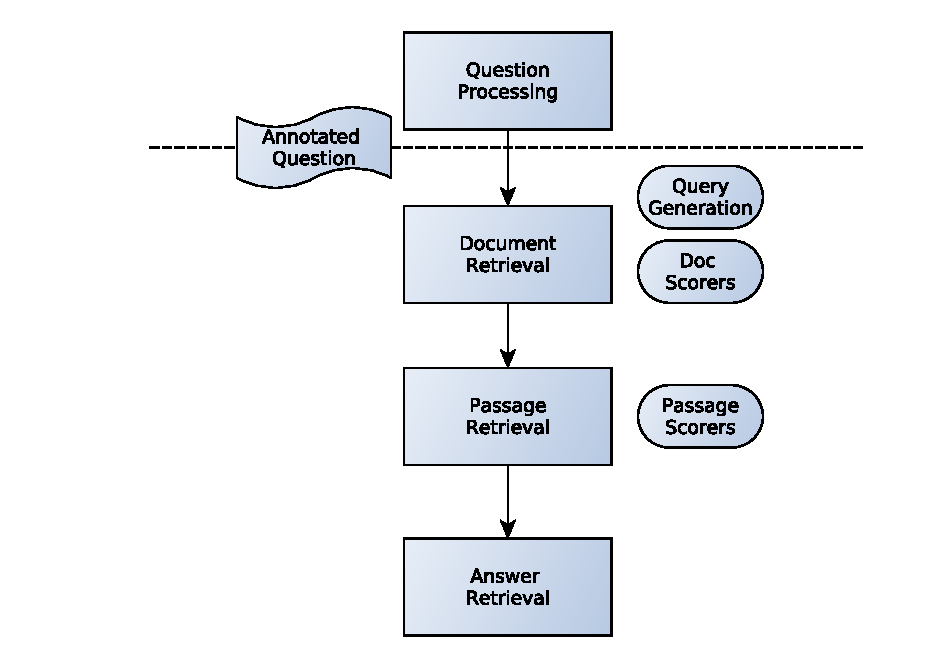
\includegraphics[scale=0.75]{graficos/AnswerRetrievalFlowWiki}
%   \caption{Flow para la Generación de Respuestas - No Estructurado}
%   \label{fig:AnswerRetrievalFlowWiki}
% \end{figure}

% \subsubsection{Documentos}
% \label{subsec:docs}
% En este punto, para una pregunta dada se dispone de la entidad del grupo de preguntas y de las distintas anotaciones hechas a la pregunta en el paso anterior (\allref{sec:qprocess}). Por su parte, los documentos en los índices invertidos poseen los campos $Id$, $Title$, y $Text$. El mecanismo de generación de queries tiene como objetivo priorizar en el ranking los documentos relacionados con el tema asociado al grupo de preguntas. Este paso es un problema de information retrieval puro: esto es, dado un pedido de información, retornar \textit{documentos relevantes}. El análisis semántico tiene peso en el paso posterior, a la hora de rankear pasajes. Por ejemplo, para el primer grupo de preguntas acerca de Harry Potter, solo se espera de este una lista de de documentos relacionados con ese mundo, en primer lugar. Por otro lado, es necesario que los principios de generación de queries no sean demasiado estrictos. Si en este punto quedan afuera muchas ocurrencias de una respuesta, entonces todo el resto del programa se ve afectado de manera irreparable. Es preferible generar documentos de más y luego filtrarlos mediante análisis lingüístico que ser demasiado estrictos y perder respuestas.
% Para lograr esto, ponderamos los documentos en los que las entidades nombradas reconocidas lingüísticamente aparecen en el título, si se dispone de más de una entidad buscamos documentos que mencionen ambos, luego priorizamos los documentos que poseen estas entidades dentro del cuerpo y también consideramos la presencia de verbos en diferentes conjugaciones y de sustantivos que ocurren en la pregunta. Finalmente, agregamos una lista de documentos enviando la pregunta misma como una query.

% Dado que finalmente se realizan queries simples (masivas), cabe preguntarse cual es la razón de la generación de queries y la ponderación de documentos. Esta razón es que en el proceso de ranking de pasajes y evaluación de respuesta se utilizan features basados en el score dado por lucene a los diferentes documentos. Si una mejor posición del documento contenedor del pasaje no implica que el pasaje sea correcto, si en cambio es un indicador de que dicho pasaje se encontró más cerca o más lejos del nucleo temático en el que se esperaba encontrarlo.

% Una vez generada la lista de documentos rankeados según lucene, se procede a analizar algunos features en base a distintos scorers propios. A su vez, estos distintos valores se combinan en una evaluación general del documento, que será utilizada luego a la hora de generar una respuesta. Estas dimensiones buscan en el título y en el artículo diferente medidas sobre las entidades nombradas y sobre la pregunta completa. En concreto, se miden distancias a la entidad nombrada que identifica al grupo de preguntas (ver \allref{subsec:entidad-de-grupo}), las entidades nombradad en la pregunta misma, a la pregunta completa y la respuesta esperada data. Las medidas contra la respuesta esperada -dada por Clef- no pueden usarse para generar la respuesta, pero sí para evaluar la performance del sistema. En el siguiente cuadro se muestran las dimensiones que se consideran sobre los documentos.

% \begin{center}
% \begin{tabular}{| l | l | l |}
% \hline
% Entidad & Campo & Comparador \\ \hline
% \multirow{6}{*}{Entidad de Grupo} & \multirow{3}{*}{Título} & Span \\
% & & Covr \\
% & & Freq \\ \cline{2-3}
% & \multirow{3}{*}{Texto} & Span \\
% & & Covr \\
% & & Freq \\ \hline
% \multirow{6}{*}{Entidades de Pregunta} & \multirow{3}{*}{Título} & Span \\
% & & Covr \\
% & & Freq \\ \cline{2-3}
% & \multirow{3}{*}{Texto} & Span \\
% & & Covr \\
% & & Freq \\ \hline
% \multirow{6}{*}{Todas las entidades} & \multirow{3}{*}{Título} & Span \\
% & & Covr \\
% & & Freq \\ \cline{2-3}
% & \multirow{3}{*}{Texto} & Span \\
% & & Covr \\
% & & Freq \\ \hline
% \multirow{6}{*}{Pregunta} & \multirow{3}{*}{Título} & Span \\
% & & Covr \\
% & & Freq \\ \cline{2-3}
% & \multirow{3}{*}{Texto} & Span \\
% & & Covr \\
% & & Freq \\ \hline
% \multirow{6}{*}{Respuesta} & \multirow{3}{*}{Título} & Span \\
% & & Covr \\
% & & Freq \\ \cline{2-3}
% & \multirow{3}{*}{Texto} & Span \\
% & & Covr \\
% & & Freq \\ \hline
% Score según índice & -- & -- \\ \hline
% \end{tabular}
% \end{center}

% Los comparadores señalados ($Freq$, $Covr$, y $Span$) se utilizan en distintos lugares de esta tesis y su funcionamiento es explicado en el apéndice \allref{sec:comparadores}. Notar que `Entidades de la pregunta' refiere tanto a aquellas reconocidas por el NER-tagger como a construcciones sustantivadas y que `Pregunta' no es la pregunta bruta sino la priorización de verbos conjugados, sustantivos, adjetivos y entidades.

% El score general del documento es un cálculo ponderado de estas diferentes dimensiones.

% Lucene permite especificar cuántos documentos queremos recuperar. Para evaluar la performance de este paso, utilizamos medida distintos scores en base a la respuesta dada por dada por la conferencia para el ejercicio. Es importante notar que dado que no utilizamos las imagenes de wikipedia de la primera sugerencia, es esperable que las respuesta no estén `tal cual'.
% Evaluamos distintos mecanismos de generación de documentos, con distinta cantidad total, bajo distintas métricas. Para generar documentos, probamos la query trivial $ALL: pregunta$ (1), una un poco mejorada $ALL: entidad_de_grupo pregunta$ (2), secuencias concatenadas de queries tal como las describimos más arriba (3) y varios pedidos separados aplanados en un paso posterior (4). Para los cuatro métodos eliminamos los signos de puntuación. Para medir los resultados, utilizamos los comparadores de presencia exacta y diferentes grados de cobertura de términos (.8, .9 y 1). A su vez, evaluamos distintas imagenes de wikipedia para el español. Es total de preguntas del ejercicio, recordamos, es 200. Los resultados son los siguientes.

% \begin{center}
% \begin{tabular}{|l|l|l|l|l|l|l|}
% \hline
% Método & \# Docs & Wikipedia & Exacto & Covr 1 & Covr .9 & Covr . 8 \\ \hline

% \multirow{6}{*}{1 - Trivial} &
% \multirow{3}{*}{100} & es - 2006 & 132 & 151 & 152 & 159 \\
%  &  & es - 2007 & 144 & 159 & 160 & 164 \\
%  &  & en - 2006 & x & x & x & x \\ \cline{2-7}
%  & \multirow{3}{*}{1000} & es - 2006 & 144 & 167 & 167 & 173 \\
%  &  & es - 2007 & 159 & 177 & 177 & 180 \\
%  &  & en - 2006 & x & x & x & x \\ \hline

% \multirow{6}{*}{2 - Trivial'} &
% \multirow{3}{*}{100} & es - 2006 & 138 & 156 & 157 & 164 \\
%  &  & es - 2007 & 151 & 167 & 168 & 171 \\
%  &  & en - 2006 & x & x & x & x \\ \cline{2-7}
%  & \multirow{3}{*}{1000} & es - 2006 & 147 & 168 & 168 & 174 \\
%  &  & es - 2007 & 163 & 178 & 178 & 181 \\
%  &  & en - 2006 & x & x & x & x \\ \hline
% hola & ey &wiki& 137 & 156 & 157 & 160  \\ \hline
% \multirow{6}{*}{3 - Inteligente} &
% \multirow{3}{*}{100} & es - 2006 & 127 & 144 & 144 & 150 \\
%  &  & es - 2007 & 141 & 150 & 151 & 156 \\
%  &  & en - 2006 & x & x & x & x \\ \cline{2-7}

%  & \multirow{3}{*}{1000} & es - 2006 & 143 & 163 & 163 & 170 \\
%  &  & es - 2007 & 158 & 175 & 175 & 179 \\
%  &  & en - 2006 & x & x & x & x \\ \hline

% \multirow{6}{*}{4 - Inteligente'} &
% \multirow{3}{*}{100} & es - 2006 & 142 & 160 & 161 & 168 \\
%  &  & es - 2007 & 157 & 170 & 171 & 174  \\
%  &  & en - 2006 & x & x & x & x \\ \cline{2-7}


%  & \multirow{3}{*}{1000} & es - 2006 & 147 & 168 & 168 & 174 \\
%  &  & es - 2007 & x & 158 & x & x \\
%  &  & en - 2006 & x & x & x & x \\ \hline

% \end{tabular}
% \end{center}

% Conclusión de esto.

% \subsubsection{Pasajes}
% Este paso es análogo al anterior, pero con mayor detalle y granularidad. Cada documento generado en el paso anterior, con sus diferentes puntajes para
% las dimensiones señaladas, se parten en pasajes u oraciones. Nuevamente, sobre estas oraciones realizamos diferentes mediciones y las combinamos generando
% un score final. En esta sección discutiremos las mediciones consideradas y los diferentes métodos de combinación de las mismas. Estos métodos de combinación generan distintos rankings de pasajes. Para evaluar estos rankings, nuevamente, utilizaremos la información disponible sobre las respuestas esperadas, buscando que la respuesta esperada se encuentre entre los $n$ pasajes mejor rankeados.
% En primer lugar, las distintos scorers implementados son los siguientes:

% \begin{center}
% \begin{tabular}{| l | l | l |}
% \hline
% Comparador & Qué & Dónde \\ \hline
% \multicolumn{3}{|c|}{Estadísticos} \\ \hline
% Freq & Pregunta & Pasaje \\ \hline
% Span & Pregunta & Pasaje \\ \hline
% Covr & Pregunta & Pasaje \\ \hline
% \#Tokens & -- & Pasaje \\ \hline
% \multicolumn{3}{|c|}{Basados en NLP} \\ \hline
% Presencia & Entidad de Grupo & Pasaje \\ \hline
% Presencia & Entidades de pregunta & Pasaje \\ \hline
% Presencia & Verbos de pregunta & Pasaje \\ \hline
% Presencia & Sustantivos de pregunta & Pasaje \\ \hline
% \multicolumn{3}{|c|}{Para evaluación} \\ \hline
% Freq & Respuesta & Pasaje \\ \hline
% Span & Respuesta & Pasaje \\ \hline
% Covr & Respuesta & Pasaje \\ \hline
% \end{tabular}
% \end{center}

% A estos Scorers se le suman los scores del documento asociado al pasaje (ver \allref{subsec:docs}).
% Sobre estas dimensiones disponibles, intentamos las siguientes combinaciones de priorización:

% \begin{center}
% \begin{tabular}{|l|l|l|}
% \hline
% \#& Nombre & Fórmula \\ \hline
% 1& Simple & $2+2=4$ \\ \hline
% 2& Respuesta & $2+2=4$ \\ \hline
% 3& Compleja & $2+2=4$ \\ \hline
% \end{tabular}
% \end{center}

% Y consideramos la ocurrencia de respuestas, de la misma manera que en el apartado anterior (Match Exacto y tres medidas de covertura de tokens: 1, .9 y .8),
% sobre los primeros $n$ pasajes, con $n$ = 1, 5, 10, 20, 50 y 100.

% \begin{center}
% \begin{tabular}{|l|l|l|l|l|l|}
% \hline
% Fórmula & \#Docs & Exacto & Covr 1 & Covr .9 & Covr . 8 \\ \hline
% \multirow{6}{*}{1} & 1 & x & x & x & x \\  \cline{2-6}
%  & 5 & x & x & x & x \\ \cline{2-6}
%  & 10 & x & x & x & x \\ \cline{2-6}
%  & 20 & x & x & x & x \\ \cline{2-6}
%  & 50 & x & x & x & x \\ \cline{2-6}
%  & 100 & x & x & x & x \\ \hline
% \end{tabular}
% \end{center}


% \subsubsection{Respuestas}





% \begin{figure}
%   \centering
%     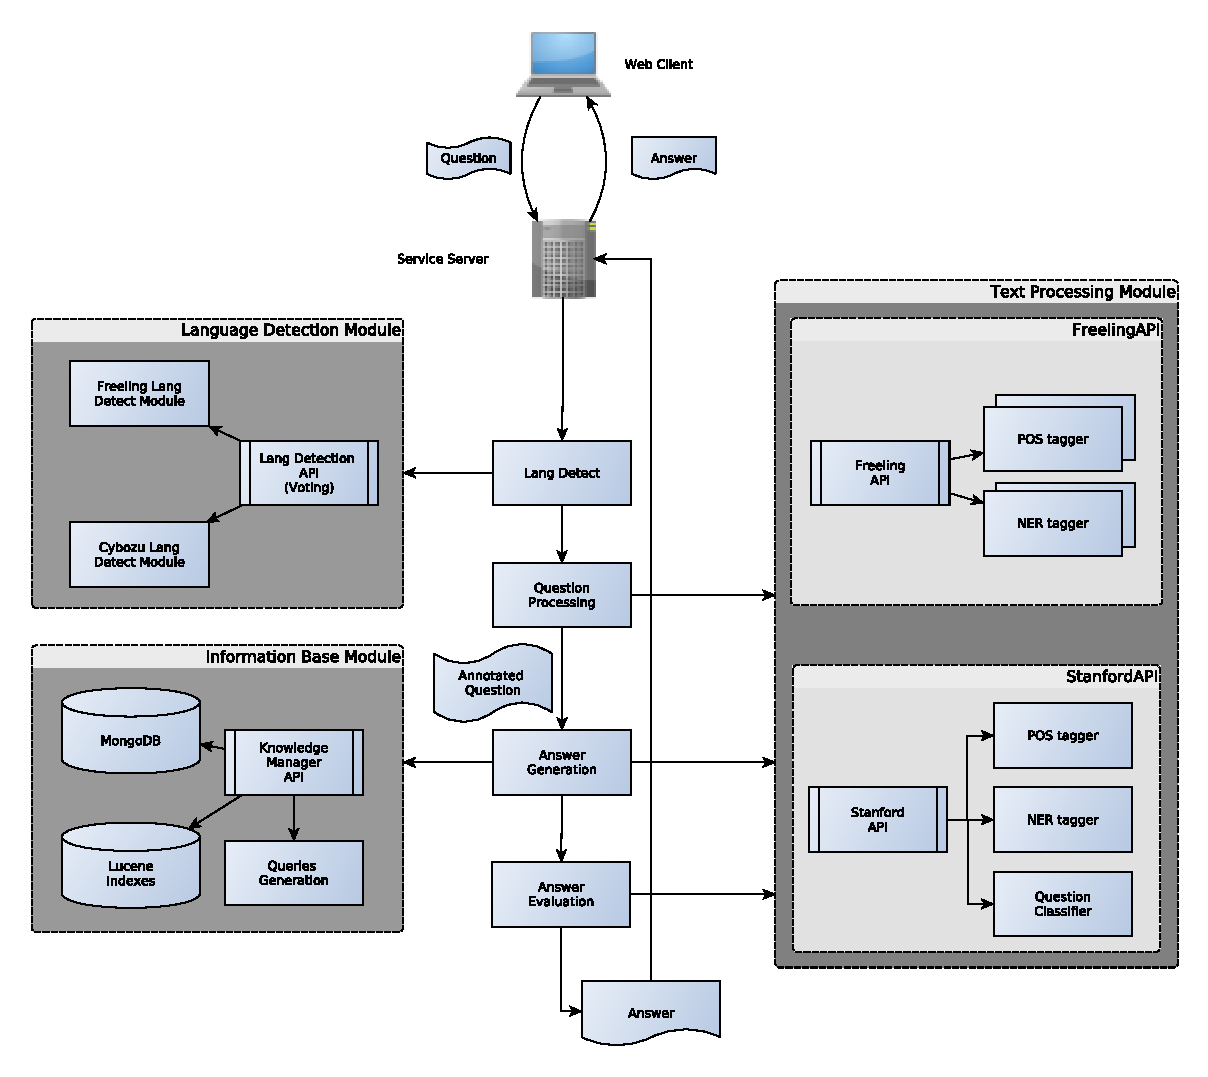
\includegraphics[scale=0.86]{graficos/Architecture}
%   \caption{Arquitectura}
%   \label{fig:Architecture}
% \end{figure}

% %\end{document}
